%
% File acl2020.tex
%
%% Based on the style files for ACL 2020, which were
%% Based on the style files for ACL 2018, NAACL 2018/19, which were
%% Based on the style files for ACL-2015, with some improvements
%%  taken from the NAACL-2016 style
%% Based on the style files for ACL-2014, which were, in turn,
%% based on ACL-2013, ACL-2012, ACL-2011, ACL-2010, ACL-IJCNLP-2009,
%% EACL-2009, IJCNLP-2008...
%% Based on the style files for EACL 2006 by 
%%e.agirre@ehu.es or Sergi.Balari@uab.es
%% and that of ACL 08 by Joakim Nivre and Noah Smith

\documentclass[11pt,a4paper]{article}
\usepackage[hyperref]{acl2020}
\usepackage{times}
\usepackage{latexsym}

\renewcommand{\UrlFont}{\ttfamily\small}
\usepackage{amsmath,amsthm,amssymb}

% This is not strictly necessary, and may be commented out,
% but it will improve the layout of the manuscript,
% and will typically save some space.
\usepackage{microtype}

\usepackage{paralist}
\usepackage{verbatim}
\usepackage[normalem]{ulem}
\usepackage[vlined,ruled,linesnumbered]{algorithm2e}
\usepackage{makecell}
\usepackage{txfonts}
\usepackage{xspace}
\usepackage{booktabs}
\usepackage{graphicx}
\usepackage{xcolor}
\usepackage{color,soul}

\usepackage[T1]{fontenc}
\usepackage{bbold}
\usepackage{pifont}% http://ctan.org/pkg/pifont


\aclfinalcopy % Uncomment this line for the final submission
%\def\aclpaperid{***} %  Enter the acl Paper ID here

%\setlength\titlebox{5cm}
% You can expand the titlebox if you need extra space
% to show all the authors. Please do not make the titlebox
% smaller than 5cm (the original size); we will check this
% in the camera-ready version and ask you to change it back.
\renewcommand{\ttdefault}{txtt}
\newcommand\BibTeX{B\textsc{ib}\TeX}
%\newcommand*{\emailfont}{\fontfamily{pcr}\selectfont}

\DeclareMathOperator*{\argmax}{arg\,max}
\DeclareMathOperator*{\argmin}{arg\,min}


\newcommand{\colbox}[2]{
\begingroup
  \setlength{\fboxsep}{0pt}%  
  \colorbox{#1}{#2\/}%\reducedstrut
\endgroup}

 
\newcommand{\veryshortarrow}[1][3pt]{\mathrel{%
   \hbox{\rule[\dimexpr\fontdimen22\textfont2-.2pt\relax]{#1}{.4pt}}%
   \mkern-4mu\hbox{\usefont{U}{lasy}{m}{n}\symbol{41}}}}
   
  
\definecolor{caddback}{rgb}{0.90, 0.98, 0.96}
\definecolor{cadd}{rgb}{0, 0.47, 0.34}
\definecolor{cdelback}{rgb}{1, 0.94, 0.92}
\definecolor{cdel}{rgb}{0.83, 0.32, 0.16}
\def \arrow{$\veryshortarrow$}
\newcommand{\add}[1]{\colbox{caddback}{{\color{cadd}#1\xspace}}} %
\newcommand{\remove}[1]{\colbox{cdelback}{{\color{cdel}#1\xspace}}}%
\newcommand{\swap}[2]{\remove{#1} \arrow\add{#2}}
\newcommand{\changed}[2]{{#1}\arrow ~\add{#2}}
\newcommand{\ctrltag}[1]{\texttt{#1}\xspace}


\definecolor{cexample}{rgb}{0.23, 0.30, 0.45}
\newcommand{\exinline}[1]{ {\color{cexample}``#1''\xspace}}
\newcommand{\fillin}[1]{ {\color{cexample}#1\xspace}}

\newcommand{\fontsmall}{\fontsize{9pt}{11pt}\selectfont}
\newcommand{\fontnormal}{\fontsize{10pt}{12pt}\selectfont}
\fboxrule=0.1pt
\newcommand{\ebox}[1]{%
	\medskip
	\noindent\fcolorbox{gray}{white}{
		\begin{minipage}{0.95\linewidth}
			\fontsmall
			%\begin{internallinenumbers}
			%\resetlinenumber
			{#1}
			%\end{internallinenumbers}
		\end{minipage}
	}
	\medskip
}

% [(0.166, 'opposing '), (0.099, 'team '), (0.027, 'by '), (0.026, 'quarterback '), (0.024, 'The '), (0.024, 'is '), (0.024, '. '), (0.023, ' '), (0.023, 'about '), (0.023, 'to '), (0.023, 'be '), (0.023, 'tackled '), (0.019, 'the '), (-0.0, ' ')]
%#eef5fa
%#daeaf5
%#c6deef
%#b2d2e9
%#9ec7e4
%#8abbde

\definecolor{cfwone}{HTML}{eef5fa}
\definecolor{cfwtwo}{HTML}{daeaf5}
\definecolor{cfwthree}{HTML}{b2d2e9}
\definecolor{cfwfour}{HTML}{8abbde}

\newcommand{\fwone}[1]{\colbox{cfwone}{#1}\xspace}
\newcommand{\fwtwo}[1]{\colbox{cfwtwo}{#1}\xspace}
\newcommand{\fwthree}[1]{\colbox{cfwthree}{#1}\xspace}
\newcommand{\fwfour}[1]{\colbox{cfwfour}{#1}\xspace}

\newcommand{\fexp}[2]{\texttt{{\color{darkgray}{#1:#2}}}\xspace}
\newcommand{\fexptag}[1]{\fexp{TAG}{#1}}
\newcommand{\fexpfrom}[1]{\fexp{FROM}{#1}}
\newcommand{\fexpto}[1]{\fexp{TO}{#1}}


\definecolor{ctemplate}{rgb}{0.23, 0.30, 0.45}
%\definecolor{ctemplate}{rgb}{0.23, 0.30, 0.45}
\definecolor{cword}{rgb}{0, 0, 0.7}
\newcommand{\BLANK}{\texttt{ {\color{cword}[BLANK]} }}

% format
\newcommand{\clabel}[1]{\emph{#1}\xspace}

% constants
\newcommand{\sysname}{Aditor\xspace}

\newcommand{\mturkurl}{\url{https://tongshuangwu.github.io/perturb-exp-ui/?assignmentId=1&platform=standalone&debug=debug&task=nli}}
\newcommand{\tagstr}{control code\xspace}
\newcommand{\Tagstr}{Control code\xspace}
\newcommand{\tagstrs}{control codes\xspace}


\newcommand{\cmark}{{\ding{51}}}%
\newcommand{\xmark}{{\ding{55}}}%
\newcommand{\qmark}{{\textsf{?}}}%

\newcommand{\perturbtoken}{\texttt{<|perturb|>}\xspace}%
\newcommand{\stoptoken}{\texttt{[SEP]}\xspace}%



\newcommand{\eg}{\emph{e.g.,}\xspace}%
\newcommand{\ie}{\emph{i.e.,}\xspace}

% tasks
\newcommand{\nli}{NLI\xspace}
\newcommand{\sst}{Sentiment\xspace}
\newcommand{\qqp}{QQP\xspace}

\def \dsst{SST-2\xspace}
\def \dqqp{QQP\xspace}
\def \dnli{SNLI\xspace}

% annotations
\newcommand{\note}[2]{\xspace{\color{#1}[ #2 ]}\xspace}
%\newcommand{\note}[2]{}
\newcommand{\wts}[1]{\note{violet}{Sherry: #1}}









% teal, cyan
\title{\sysname: Towards Automated Perturbation Generation \\for Evaluation, Data Augmentation, and Explanation}
\begin{comment}
\author{
Tongshuang Wu \\
  University of Washington \\
  \texttt{wtshuang@uw.edu} \\\And
Marco Tulio Ribeiro \\
  Microsoft Research \\
  \texttt{marcotcr@gmail.com} \\\And
Jeffrey Heer \\
  \texttt{jheer@uw.edu} \\\And
Jeffrey Heer \\
  \texttt{jheer@uw.edu} \\
}
\end{comment}

\author{
\makecell{
Tongshuang Wu$^{1}$ ~~~~~~~ 
Marco Tulio Ribeiro$^{2}$ ~~~~~~~ 
Jeffrey Heer$^{1}$ ~~~~~ 
Daniel S. Weld$^{1}$}  \\ 
$^{1}$Allen School, University of Washington\hspace{5mm}
$^{2}$Microsoft Research\hspace{5mm} \\ 
\href{mailto:wtshuang@cs.uw.edu}{\texttt {wtshuang@cs.uw.edu}}
\hspace{2mm}
\href{mailto:marcotcr@microsoft.com}{\texttt {marcotcr@gmail.com}}
\hspace{2mm}
\href{mailto:dan@cs.washington.edu}{\texttt {\{jheer,weld\}@cs.uw.edu}}
}


\date{}

\begin{document}
\maketitle
\begin{abstract}
Minimal perturbations is effective for evaluating and calibrating model decision boundaries, but existing generation methods either cover limited linguistic patterns, or are hard to scale.
We explore language-model based perturbation generation.
We define the training prompts with two information:
To enable targeted inspection, we use \emph{\tagstrs} to indicate \emph{how} to change a sentence with defined based on common linguistic capabilities, and \emph{where} to change by blanking certain linguistic features.
We finetune GPT-2 on a combination of multiple existing datasets,  and verify its usefulness of the generations in three applications:
(1) As contrast sets, the model performance decreases up to \wts{X\%} on them compared to on the original test set, revealing model inefficiencies.
(2) As counterfactual data augmentation, they improve models on data slices, and models perform better on out-of-domain datasets, challenge sets, or pass more behavioral tests.
\wts{Number?}
(3) They also supply existing explanations and more effectively demonstrate the impact certain text.
\end{abstract}

\section{Introduction}
\label{sec:intro}



Counterfactual reasoning --- mentally simulating what \emph{would have happened} if conditions were different --- is a common tool for making causality assessments~\cite{kahneman}, which in turn are crucial for model training, evaluation, error analysis, and explanation~\cite{miller}. 
For example, in Figure~\ref{fig:teaser}, \exinline{It is great for kids} is perturbed into multiple variations, each providing unique insights by simulating what would have happened if the sentence was different.

Applications of counterfactual reasoning to NLP generally specify the relationship $x \veryshortarrow \xp$, and then create $\xp$ according to the relationship.
As a result, prior work has tailored counterfactual generators for many different applications, only collecting subsets of useful $\xp$.
%inducing different limitations.
%For example, a minimal edit of a sentence $x$ that results in a different label is useful for model training and evaluation.
%Such counterfactuals are usually produced manually by human annotators ~\cite{gardner2020contrast} or by human-written perturbation functions~\cite{wu2019errudite}, making them costly to generate (\eg 4-5 minutes per counterfactual~\cite{kaushik2019learning}) and liable to systematic omissions (\eg human annotators may miss \swap{kids}{no one} in Figure~\ref{fig:teaser}B). %Further, relying on human creativity may cause important but non-obvious patterns to be missed, \eg humans may cover \swap{great}{not great}, but miss \swap{kids}{no one} in Figure~\ref{fig:teaser}B.
%Though it is cheaper to automate the process with parsing templates~\cite{li2020linguistically}, the templates usually have limited coverage on either the patterns-to-perturb, or the applicable data points.
%In contrast, adversarial examples specify a very different counterfactual relationship: $x$ and $\xp$ must have different model predictions \emph{despite} being semantically equivalent, such that automated methods often rely on paraphrasing models~\cite{iyyer2018adversarial,  ribeiro2018semantically}.
For example, to support {\em model training and evaluation}, human annotators create counterfactuals that change the groundtruth labels by manually rewriting instances~\cite{gardner2020contrast} or defining perturbation functions~\cite{checklist:acl20}.
Manual rewrites are costly (\eg 4--5 minutes per counterfactual~\cite{kaushik2019learning}) and susceptible to systematic omissions (\eg human annotators may cover \swap{great}{not great}, but miss \swap{kids}{no one} in Figure~\ref{fig:teaser}B).
Meanwhile, automated generators aiming for \emph{model analysis and explanation} usually focus on another relationship, \ie generating $\xp$ that have different model predictions than $x$~\cite{ross2020explaining, Zhang2019GeneratingFA}. 
As a result, they neglect prediction-preserving counterfactuals that are equally important for understanding or shaping model behaviors, like \swap{kids}{no one} and \swap{great}{scary} linked to Figure~\ref{fig:teaser}D.


%In contrast, adversarial examples\dan{now you come to another use case, but 'adversarial examples' is 1) not a reason or use for Cfs; it's a characterization of theirs style, 2) it doesn't match the list of uses cases you've lined up above and (crucially) in fig 1, so 3) it doesn't reinforce Fig 1, which is the central framing of the paper. I suggest you rewrite to follow the use cases. It really matters to explain the motivation of thge paper simply and clearly and to repeat it (in a non annoying way) - avoids confusion} specify a different relationship: $x$ and $\xp$ must have the same groundtruth but different model predictions, driving the generator to prioritize paraphrasing~\cite{iyyer2018adversarial, ribeiro2018semantically}, over the non-paraphrasing changes that still preserve the groundtruth~\cite{li2020contextualized}.
%(\eg changing movie names in sentiment analysis).

\begin{figure}[t]
\centering
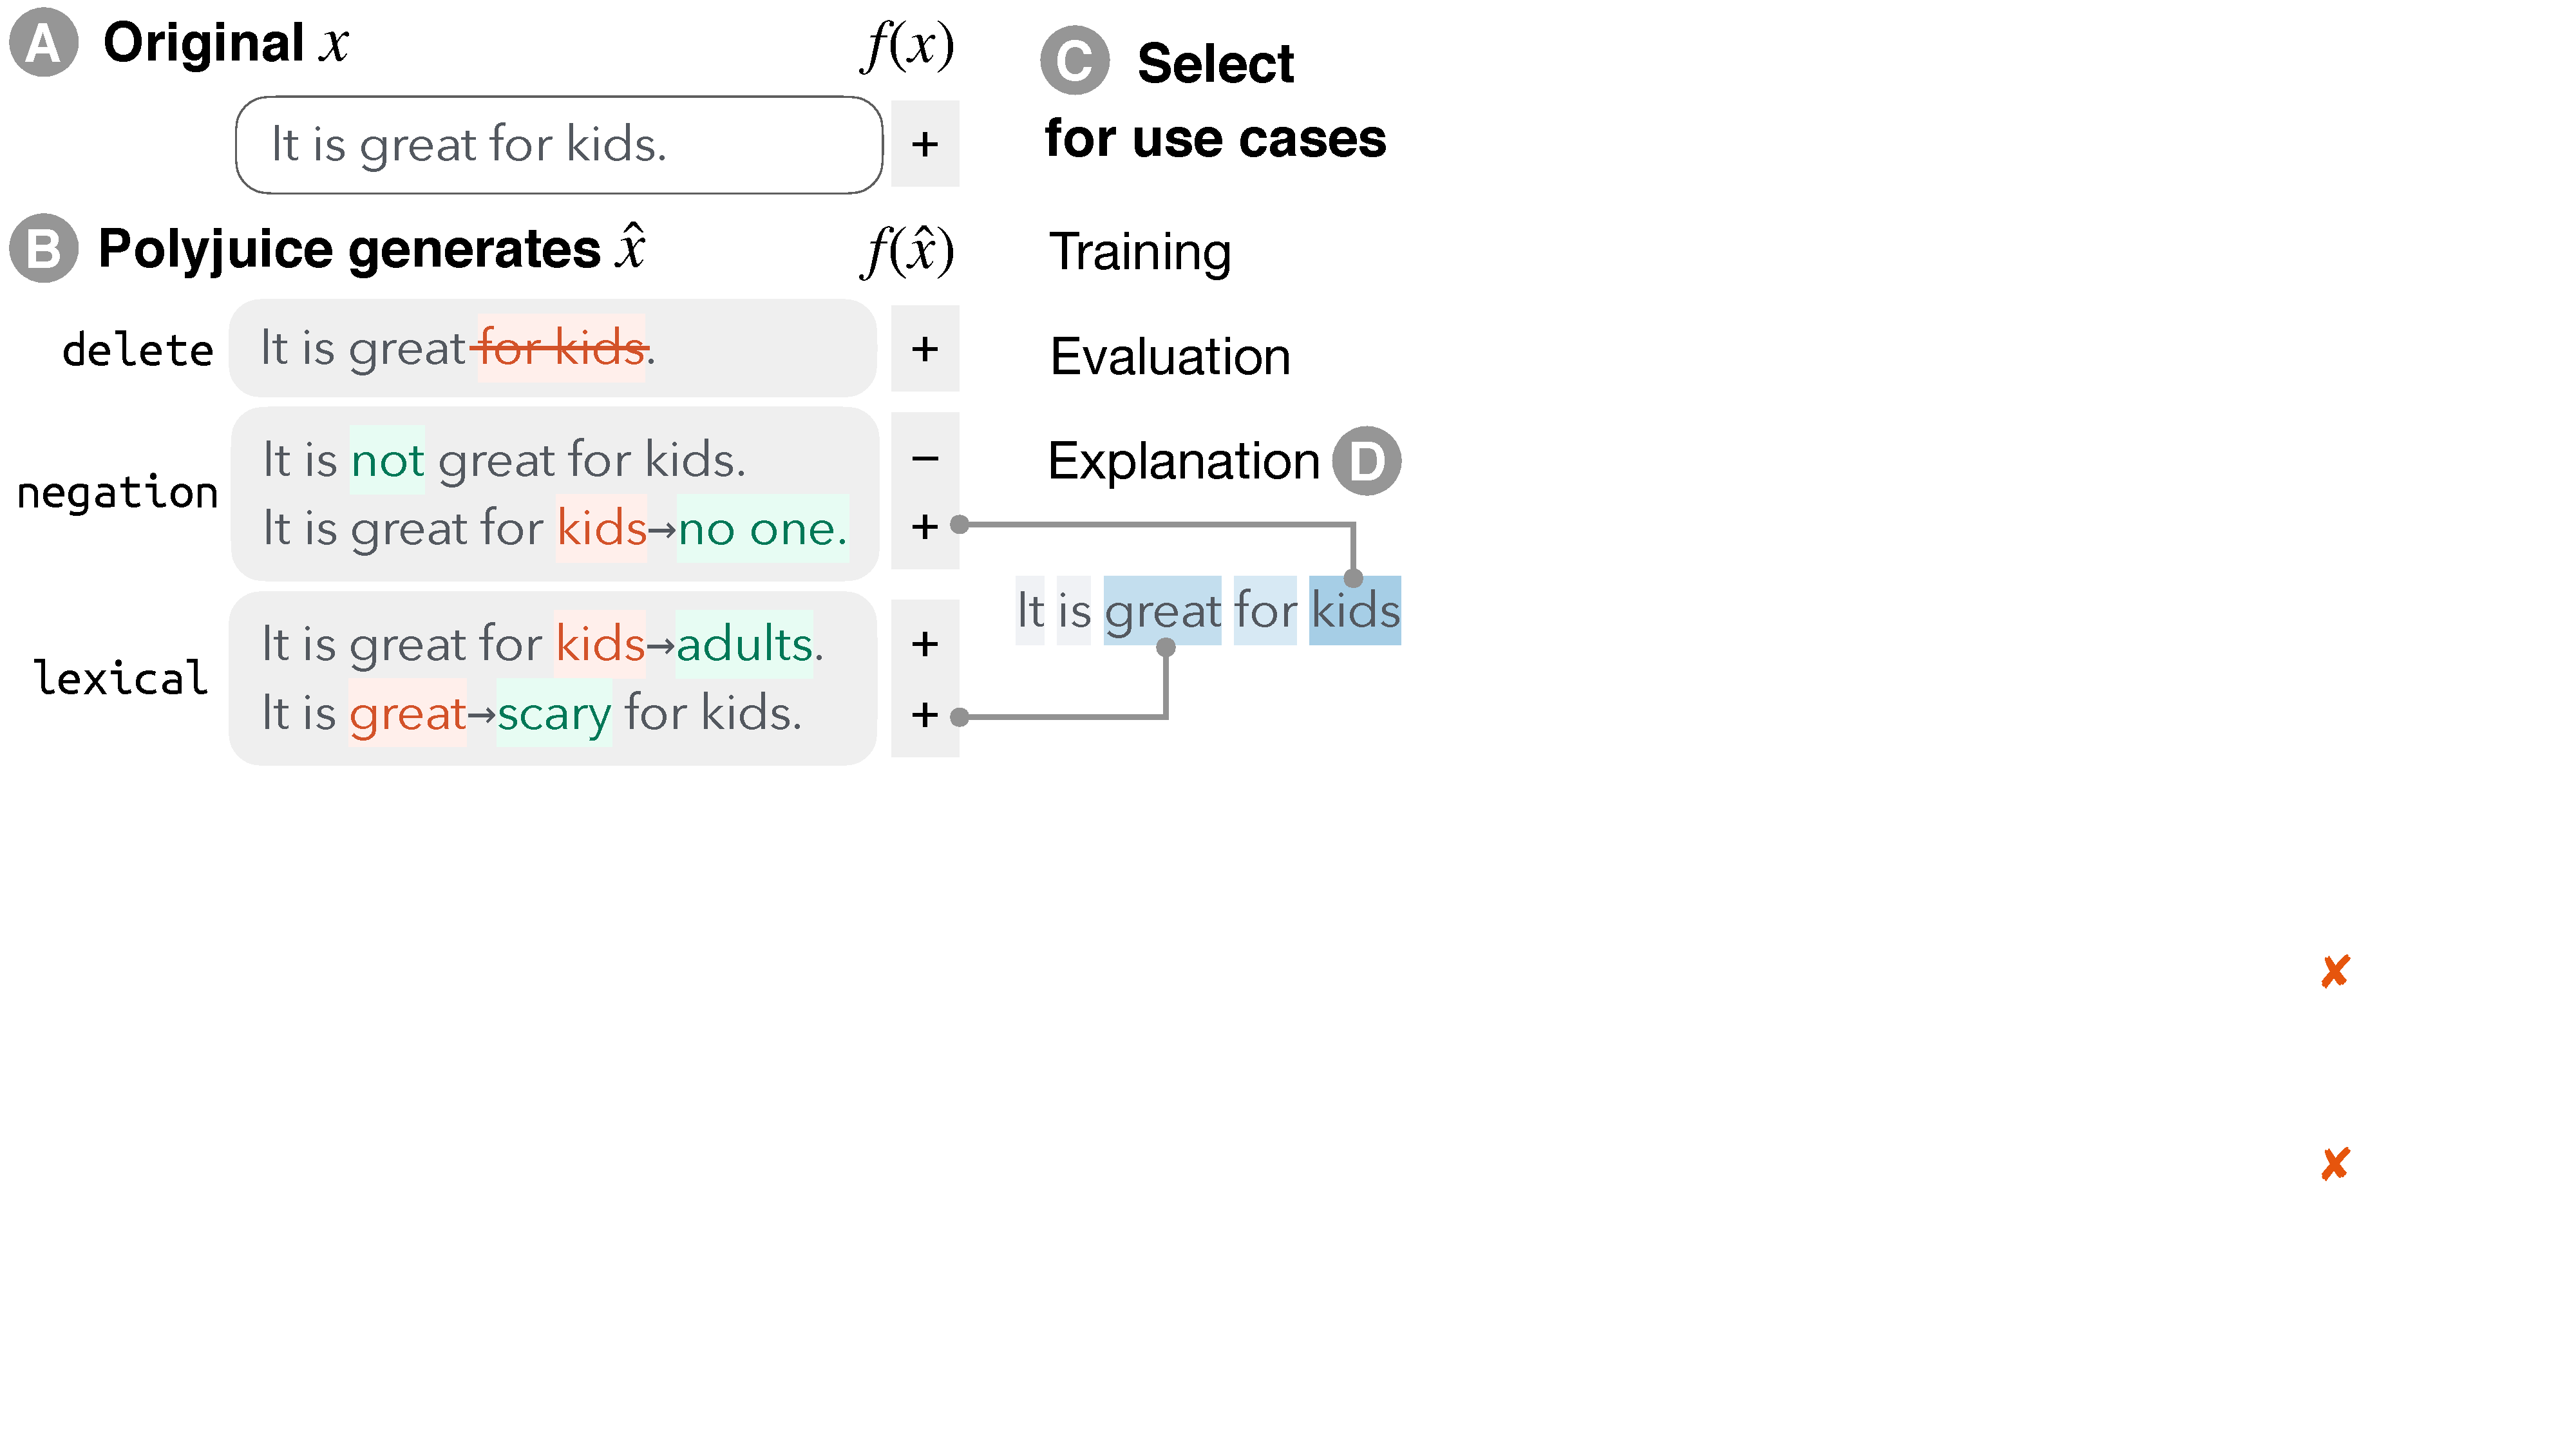
\includegraphics[trim={0 18cm 30.5cm 0cm},clip, width=1\columnwidth]{figures/teaser.pdf}
\vspace{-15pt}
\caption{
Overview: (A) given a sentiment analysis instance $x$, \sysname generates (B) various counterfactuals $\xp$, which are then (C) selected for downstream use.
\eg in (D) we select counterfactual explanations that complement a black box explanation: though ``great'' and ``kids'' are deemed important, perturbing them may not affect the prediction $f(x)=f(\xp)=\text{\emph{positive}}$, revealing model failures not covered by feature attributions.\footnotemark
}
\vspace{-10pt}
\label{fig:teaser}
\end{figure} 
\footnotetext{We open source both the \sysname model and the selection heuristics at \modelurl.}


%However, as Figure~\ref{fig:teaser} illustrates, counterfactual generation does not \emph{have} to be task-specific, as various applications share similar requirements on $x\veryshortarrow\xp$ (\eg a preference for small changes).
%In fact, a general-purpose pool of diverse counterfactuals may be preferable when the relationship is not precisely defined in advance, as is the case for counterfactual training, evaluation, or explanations.
% In fact, a common pool of counterfactuals may support each application more comprehensively.
% For example, without the preset constrain on semantic equivalence, we can collect adversarials through negation (for tasks insensitive to negation, \eg named entity recognition.)
%For example, some forms in training and evaluation data collection can 
%The exhaustive search of automated methods can cover the training and evaluation more comprehensively, and non-paraphrasing changes like \emph{add negation} are valuable adversarials for tasks like named entity recognition. 
%\hao{might be good to clarify that these two are not mutually-exclusive: adversarial examples should sometimes be close to the original}
% 
However, counterfactual generation does not \emph{have} to be task-specific.
The same set of counterfactuals in Figure~\ref{fig:teaser} can support a variety of applications.
Moreover, for cases like model explanation and analysis, a general-purpose pool of counterfactuals is preferable, as the relationship-of-interest can be more exploratory and user-oriented~\cite{wu2019errudite}.
In this work, we formalize the task of \emph{counterfactual generation}, disentangling generation from the application of counterfactuals (\S\ref{sec:general_purpose}).
Given an input $x$, our generator produces a set of counterfactuals $\hat{\xset} = \{\xp_1, \xp_2, ...\}$ with \emph{application-agnostic} relationships $x \veryshortarrow \xp_i$ (Figure~\ref{fig:teaser}B).
Afterwards, we use \emph{application-specific} selection methods to find subsets of $\xp$ that are most effective for a given use case (Figure~\ref{fig:teaser}C).

We frame the generation step as conditional text generation, and finetune GPT-2~\cite{radford2019language} into a generator called \emph{\sysname} using $(x, \xp)$ pairs. 
To allow for targeted counterfactuals, we also design \tagstrs like \ctrltag{negation} or \ctrltag{delete} (Figure~\ref{fig:teaser}B), and adopt fill-in-the-blank structures~\cite{donahue2020enabling} to specify where the perturbation occurs and how.
%We also allow for targeted counterfactuals, by specifying where the perturbation occurs~\cite{donahue2020enabling} and designing \tagstrs like \ctrltag{negation} or \ctrltag{delete} (Figure~\ref{fig:teaser}B).
Intrinsic evaluation shows that \sysname generates $\xp$ that are \emph{fluent}, \emph{diverse}, and \emph{close to $x$}, and that the \emph{control} mechanisms effectively retrieve perturbations that are rare to sample from off-the-shelf language models. %(\eg 42\% more negations).

%--- the control is \emph{the backbone of} various downstream applications.

%We propose simple yet effective selection strategies, 
With simple selection heuristics, we show that a single \sysname model can significantly aid humans in diverse downstream applications.\footnote{We demonstrate \sysname in semi-automatic settings, but as discussed in \S\ref{subsec:nlg}, it can also work automatically.} 
For \emph{counterfactual training and evaluation} (\S\ref{sec:app_label}), humans label \sysname counterfactuals rather than creating them from scratch.
They produce training data that significantly improves model generalization, as well as contrast sets that help identify model vulnerabilities~\cite{gardner2020contrast}, with 40--75\% less annotation effort. 
In another application, \sysname produces \emph{counterfactual explanations} (\S\ref{sec:app_explain}), bringing significant insight on top of state-of-the-art explanation techniques. 
Finally, \sysname supports counterfactual \emph{error analysis} (\S\ref{sec:app_err_analysis}).
It allows users to explore related counterfactuals (\eg the model responds differently to different negation forms in Figure~\ref{fig:teaser}B), and to aggregate individual counterfactuals into patterns, gaining systematic understanding of model behavior. 

%First, 
% By lifting the burden of manual rewrite, \sysname \emph{facilitates effective counterfactual training and evaluation}.
% With humans only \emph{labeling} counterfactuals, we produce training data that improves model generalization, as well as high-quality contrast sets~\cite{gardner2020contrast} with 40\%--75\% less annotation effort compared to creating them from scratch~\cite{kaushik2019learning}. 
%We similarly produce training data that improves model generalization in three classification tasks. %, when compared to adding the same amount of non-counterfactual data.

% (2) 
% %Second, 
% By generating nontrivial counterfactuals beyond paraphrasing and human intuitions, \sysname helps \emph{produce counterfactual explanations} that highlight model errors obscure to humans. 
% In a user study, experts only did slightly better than random (accuracy: $55 \pm 6\%$) at predicting what a model would do on \sysname counterfactuals, even after inspecting the model on their own.
% (3) 
% %Third, 
% By rewriting each instance in multiple ways, \sysname \emph{supports more systematic error analysis}.
% Case studies demonstrate that \sysname counterfactuals help contrast model behaviors on related perturbations (\eg the model in Figure~\ref{fig:teaser} responds differently to the two negation forms.)

% We opensource both the \sysname model and the selection strategies at \modelurl.


\begin{comment}
In summary, we:
\begin{compactenum}
\item Formalize the general-purpose counterfactual generation task. 
By \emph{separating the generation from the use cases}, we generate fluent and diverse counterfactuals that bypass application-specific constraints.
%. \hao{maybe emphasize the benefits of this}
\item Finetune a generator called \sysname, by collecting paired sentences and enhancing controls with infilling structures and \tagstrs --- the control is \emph{the backbone of} various downstream applications.
%\sysname generates plausible and diverse counterfactuals, with control over where perturbations happen and what they do.
The model is at \modelurl.
%, and we plan to opensource the selection strategies.
\item Apply \sysname to \emph{model training, evaluation, and explanation}, using various selection methods (which we will opensource).
\sysname helps collect high-quality training and evaluation data with 40\% less annotation effort, and find model bugs that on top of feature attribution explanations and counterfactual analysis.
\end{compactenum}
\wts{Maybe can delete if we run out of space.}
\end{comment}

% we observe that \sysname explanations can complement popular feature attribution methods and highlight their blind spots.
% After viewing SHAP weights~\cite{NIPS2017_7062} and interacting with the model, experts still could not predict model behaviors on counterfactuals selected for explanations, and missed 5\% and 25\% more cases than the human-generated or random baselines.

\section{General-purpose Counterfactuals}
\label{sec:general_purpose}



\newcommand{\tagdefine}[1]{\emph{{\color{darkgray}#1} }}
%\renewcommand{\arraystretch}{1.1}
\newcommand{\TagTable}{
\begin{table*}
\small
\centering
\begin{tabular}{@{} p{0.11\linewidth} p{0.61\linewidth} p{0.22\linewidth} @{}}
\toprule
\textbf{\Tagstr} & \textbf{Definitions and \sysname-generated Examples} & \textbf{Training Datasets} \\ 
\midrule
\ctrltag{negation}
 & A dog is \add{not} embraced by the woman.
 &\cite{kaushik2019learning}
\\ \midrule
\ctrltag{quantifier}
 & \swap{A dog is}{Three dogs are} embraced by the woman. 
 &\cite{gardner2020contrast}
\\ \midrule
\ctrltag{shuffle}
 & \tagdefine{To move (or swap) key phrases or entities around the sentence.} \newline
 A \swap{dog}{woman} is embraced by the \swap{woman}{dog}.
 &\cite{zhang2019paws}
\\ \midrule
\ctrltag{lexical}
 & \tagdefine{Ro change just one word or noun chunks without breaking the POS tags.} \newline
 A dog is \swap{embraced}{attacked} by the woman.
 &~\cite{sakaguchi2019winogrande}
\\ \midrule
\ctrltag{resemantic}
 & \tagdefine{To replace short phrases or clauses without affecting the parsing tree.}\newline
 A dog is \swap{embraced by the woman}{wrapped in a blanket}.
 &\cite{wieting2017paranmt}
\\ \midrule
\ctrltag{insert}
 & \tagdefine{To add constraints without affecting the parsing structure of other parts.} \newline
 A dog is embraced by the \add{little} woman.
 &\cite{mccoy2019right}
\\ \midrule
\ctrltag{delete}
 & \tagdefine{To remove constraints without affecting the parsing structure of other parts.} \newline
 A dog is embraced \remove{by the woman}.
 &~\cite{mccoy2019right}
\\ \midrule
\ctrltag{restructure}
 & \tagdefine{To alter the dependency tree structure, \eg changing from passive to positive.} \newline
 A dog is \swap{embraced by}{hugging} the woman.
 &\cite{wieting2017paranmt}
\\
\bottomrule
\end{tabular}
\vspace{-5pt}
\caption{A list of \tagstrs we designed to drive the generation, their \emph{\sysname-generated} examples, and the representative training datasets for the corresponding patterns. Details are in Appendix~\ref{appendix:train_data}.
%More examples are in Appendix~\ref{appendix:example}.
}
%\wts{Change all the examples to be on an identical sentence, not all different cases. And consider further annotate the tags based on whether they just do semantic change or also syntactic change.}}
\label{table:ctrltag}
\vspace{-12pt}
\end{table*}
}
% on a particular instance
% 
\subsection{Definition and Desiderata}
\label{sec:desiderata}


Given an instance $x \in \xset$, a generator $g$ produces a set of counterfactuals $\hat{\xset} = \{\xp_1, \xp_2, ...\}$ with various relationships $x \veryshortarrow \xp_i$. % (referred as $\relation{\xp_i}$ for simplicity).
% Each $\xp_i$ perturbs $x$ with certain strategies like negations, syntactic restructuring, etc., and the edited spans are instantiations of the strategies.
For example, \swap{great}{not great}, \swap{kids}{no one} in Figure~\ref{fig:teaser}B are both instances of the \ctrltag{negation} relationship.
% The importance of certain $\relation{\xp}$ changes along with applications.
Each $(x, \xp)$ pair shares multiple relationships --- these two are also instances of the \emph{label flipping} relationship if the task is sentiment analysis (but might not be for other tasks).
As illustrated in \S\ref{sec:intro}, knowing which relationships apply aids selection for downstream applications.

We expect $g$ to produce counterfactuals $\xp$ that are (1) \textbf{close} to $x$, preferably only involving the minimal changes necessary to establish a certain effect~\cite{pearl2018causal}, allowing users to make causality assessments.
The generated $\xp$ should also be (2) \textbf{fluent}, \ie grammatically correct~\cite{morris2020textattack} and semantically meaningful (\eg \exinline{Colorless green ideas sleep furiously} is not meaningful~\cite{chomsky2002syntactic}).
Fluency operationalizes ``probable'' counterfactuals in the context of NLP;
as \citet{kahneman} stated, humans strongly favor counterfactuals that are close to the original instance, but also prefer those that could have easily happened without assuming rare events or strange coincidences.
%Humans strongly favor counterfactuals that are close to the original instance, but also prefer them to be probable, \ie they could have easily happened without assuming rare events or strange coincidences~\cite{kahneman}.
%We operationalize ``probable'' in the context of NLP by requiring $g$ to generate (2) \textbf{fluent} $\xp$, \ie grammatically correct~\cite{morris2020textattack} and semantically meaningful (\eg \exinline{Colorless green ideas sleep furiously} is not meaningful~\cite{chomsky2002syntactic}).
Further, as a general-purpose generator, $g$ should produce counterfactuals with a measure of (3) \textbf{control} over relationships $x \veryshortarrow \xp$,  %$\relation{\xp}$,
such that the counterfactuals can vary with the object-of-attention in each application (the ``focus rule''~\cite{kahneman}).
Finally, %even though infinite diverse counterfactuals can be produced~\cite{pearl2018causal},
we expect $g$ to output a (4) \textbf{diverse} set of $\xp$ in terms of relationships, covering a large variety of ``what-ifs'' for different applications~\cite{pearl2018causal}.

%A counterfactual $\xp$ should be \textbf{close} to $x$, preferably only involving the minimal changes necessary to establish a certain effect~\cite{pearl2018causal} for causality assessments about $\relation{\xp}$. 
%Humans strongly favor counterfactuals that are close to the original instance~\cite{kahneman}, while also being probable, \ie which could have easily happened without assuming rare events or strange coincidences.
%We operationalize ``probable'' in the context of NLP by requiring $\xp$ that are \textbf{fluent}, \ie grammatically correct~\cite{morris2020textattack} and semantically meaningful (\eg \exinline{Colorless green ideas sleep furiously} is not meaningful~\cite{chomsky2002syntactic}).
%A general-purpose generator should be able to generate counterfactuals with a measure of \textbf{control} over relationships $\relation{\xp}$, such that counterfactuals vary with the object of attention depending on the application at hand (the ``focus rule''~\cite{kahneman}).
%Finally, we expect the output set $\hat{\xset}$ to be \textbf{diverse} in terms of relationships, so as to support diverse applications.

% Meanwhile, we also expect to collect sets with (4) \textbf{controlled} $\relation{\xp}$ relationships.
% The control is essential to support a wide range of specific applications, \eg counterfactual explanations on salient features (\S\ref{sec:app_explain}), error analyses that group semantically or syntactically related $\xp$ (\S\ref{sec:app_err_analysis}), etc.
% It reflects the ``focus rule''~\cite{kahneman}: counterfactuals would vary with the object of attention.
%, even when the same variable is acted upon.
%Following common practice in NLP research, we estimate \emph{closeness} using the semantic and syntactic distance between $x$ and $\xp$~\cite{morris2020textattack, madaan2020generate}.
% However, $\xp$ also needs to be (2) \textbf{fluent}, \ie grammatically correct~\cite{morris2020textattack} and semantically meaningful (\eg \exinline{It's scary for water} is not meaningful.)
% This estimates the likelihood of a sentence occurring in reality; as \citet{kahneman} stated, the counterfactual scenario should be one that could have easily happened without rare assumptions. 
%In NLP, this translates to sentences that are likely to be written.


%However, $\xp$ also needs to be realistic, \ie the counterfactual scenario should be one that could have easily happened, without rare assumptions or coincidences~\cite{kahneman}. 
%In NLP, this translates to sentences that are likely to be written, \ie (2) \emph{fluent} counterfactuals that are grammatically correct~\cite{morris2020textattack} and semantically meaningful (\eg \exinline{It's scary for water} is grammatically correct but not meaningful.) 

% Since there can be an infinite number of ``what-ifs''~\cite{pearl2018causal}, we also consider properties of $\hat{\xset}$, the produced \emph{set of counterfactuals}.

% Since our goal is to produce a general-purpose set of counterfactuals, we expect the set to be (3) \textbf{diverse} in terms of relationships between $x$ and $\xp$.
%However, when the targeted relationship is unclear, an approximation could be the similarity of counterfactuals \emph{to each other} (using \eg self-BLEU~\cite{Hu2017TowardCG}).
%, and also to contain various instantiations of the same relationship.
% Meanwhile, we also expect to collect sets with (4) \textbf{controlled} $\relation{\xp}$ relationships.
% The control is essential to support a wide range of specific applications, \eg counterfactual explanations on salient features (\S\ref{sec:app_explain}), error analyses that group semantically or syntactically related $\xp$ (\S\ref{sec:app_err_analysis}), etc.
% It reflects the ``focus rule''~\cite{kahneman}: counterfactuals would vary with the object of attention.
%Additionally, augmentations usually prioritize (3) \emph{diversity} --- a group of $x$s are preturbed using various strategies, and various initiations under the same strategy, such that they provide different constraints on finetuning decision boundaries.
%On the other hand, evaluations and explanations require more (4) \emph{controlled} perturbations for systematic and targeted inspections.
%The diversity and the controllability are two competing factors, and prior work focusing on certain applications follow one of two extremes.
%Those that thrive in diversity are either too uncontrolled (\eg text generation~\cite{iyyer2018adversarial}) or hard to scale (\eg manual rewrites~\cite{kaushik2019learning, gardner2020contrast}), whereas those that rely on templates or heuristic rules usually only cover limited linguistic patterns~\cite{li2020linguistically}.


\begin{figure}[t]
\centering
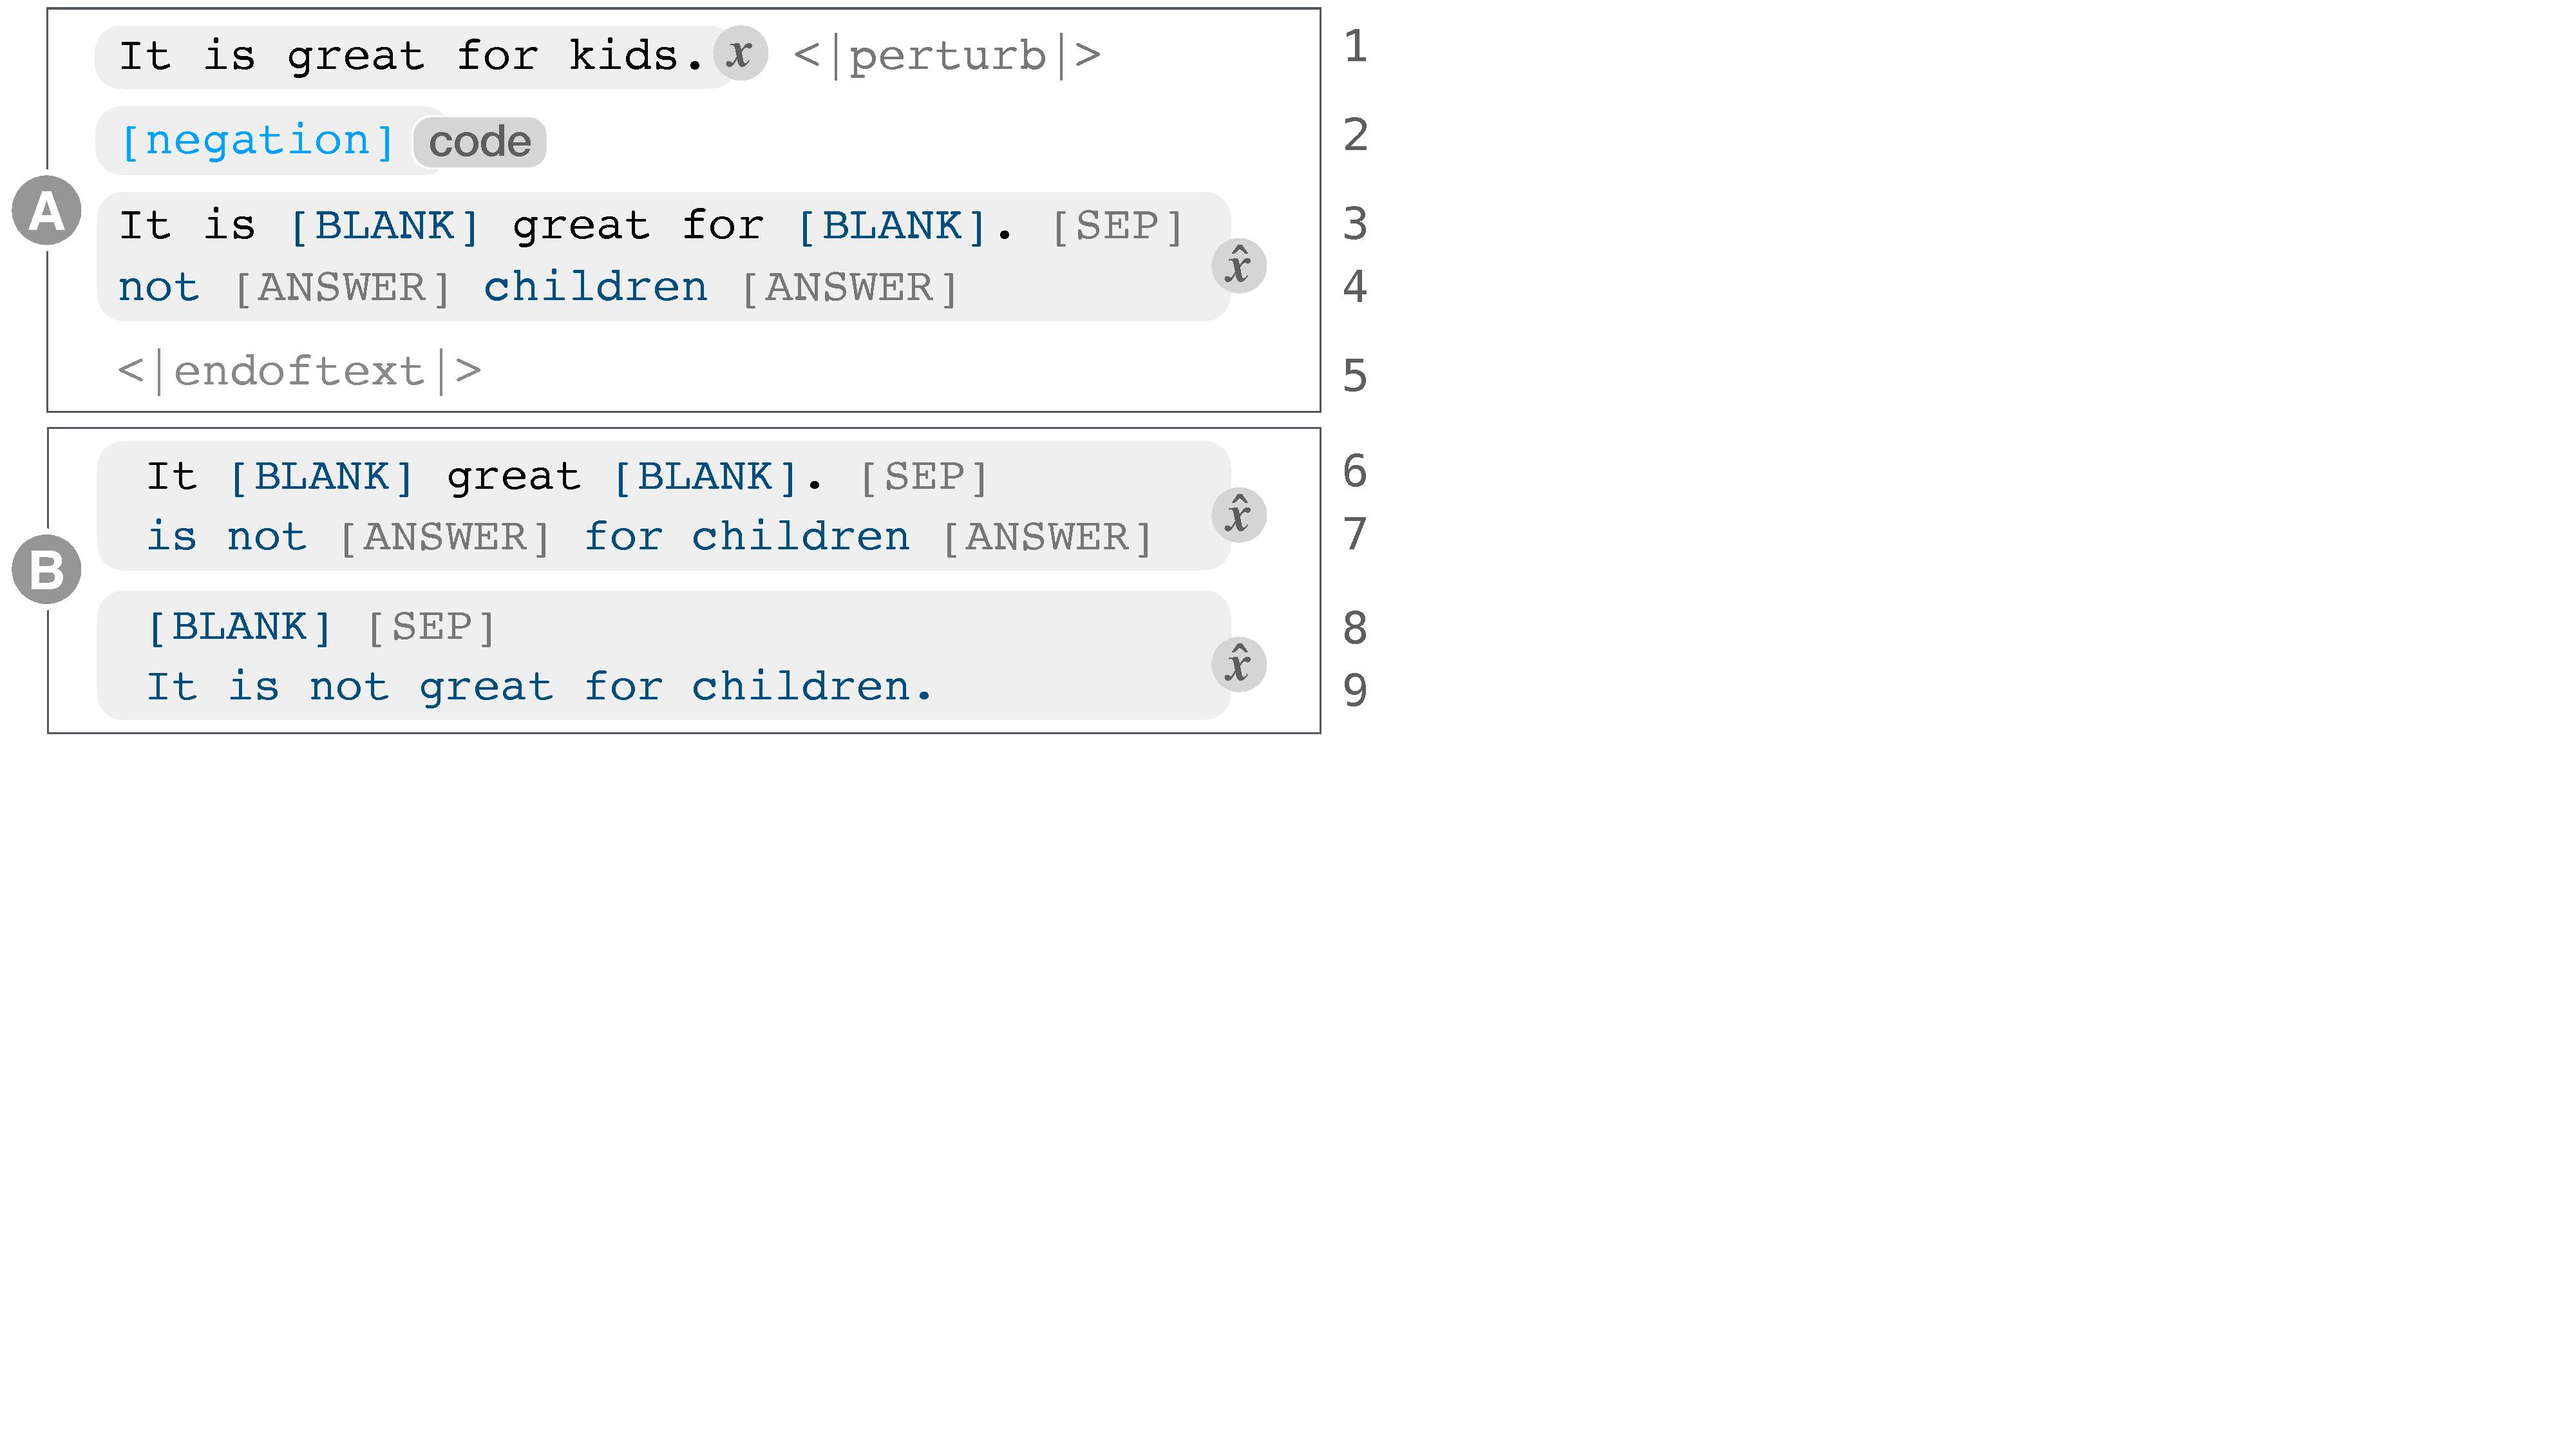
\includegraphics[trim={0 18.6cm 31.5cm 0cm}, clip, width=1\columnwidth]{figures/blank.pdf}
\vspace{-15pt}
\caption{ 
(A) \sysname prompt format, which concatenates the original $x$, the \tagstr, and the $\xp$ (\exinline{It is not great for children} converted to the infilling structure).
At \emph{generation} time, \sysname accepts prompts that just include $x$ (Line 1), or optionally with the \tagstrshort and the \texttt{[BLANK]}s (Lines 2--3), and fill in the blanks sequentially with spans separated by \texttt{[ANSWER]}s (Line 4).
%During training, the \tagstrshorts and blanks are automatically extracted.
(B) \sysname allows blanking at different granularities (even the entire sentence), such that Lines 3--4 in (A) can be replaced by Lines 6--7 or 8--9. 
%\dq{}
%We get multiple training texts per pair, by blanking $\xp$ subtrees that contain the change, or the entire sentence.
}
\vspace{-10pt}
\label{fig:blank}
\end{figure}


\subsection{Conditional Counterfactual Generation}
\label{subsec:nlg}


\TagTable

We frame counterfactual generation as a conditional text generation task using language models (LMs). To ensure that $\xp$ is \emph{close} to $x$ rather than arbitrary text, we condition the generation on $x$, followed by a special token (Line 1 in Figure~\ref{fig:blank}A).
In Line 2, we have \emph{\tagstrs} \cite{ctrl} such as \ctrltag{negation}, which specify the type of perturbation from among lexical, syntactic, or semantic \tagstrshorts (see Table \ref{table:ctrltag}), inspired by prior work that categorizes manually created counterfactuals~\cite{kaushik2019learning, gardner2020contrast}.
% All the \tagstrshorts are described in Table~\ref{table:ctrltag}. 
As an additional layer of control over $x \veryshortarrow \xp$, % $\relation{\xp}$,
we allow users to specify \emph{where} changes happen by having the LM infill \texttt{[BLANK]} tokens~\cite{donahue2020enabling}, rather than generating arbitrary counterfactuals (Lines 3--4).
At generation time, if the user provides only the original example, \sysname will generate the \tagstr, the location of blanks, and the infilling (Lines 2--4). 
Alternatively, the user can specify the \tagstr, or the \tagstr \emph{and} the location of the blanks, to exercise different degrees of control depending on the application.

% \paragraph{\emph{Closeness} and \emph{Controllability}: Conditional text generation.}
%1. We frame it as conditional text generation. We always condition on the original x (Line 1)
%2. Control codes: explain what they are , reference table 1, etc (Line 2)
%3. Blanking: we extend ILM, etc. This is why it's nice, etc (Line 3).
%4. Control codes & blanking allow for control, but they are optional: the generator can generate them based on the original x

% We frame counterfactual generation as a conditional text generation task using language models (LMs), and wrap the \emph{conditions} into textual prompts as in Figure~\ref{fig:blank}.
% First, to ensure $g$ generates $\xp$ that are \emph{close} to $x$ (rather than arbitrary text), we build mappings between paired, and always condition the generation on the original $x$ (Line 1).

% Second, to achieve the control on $\relation{\xp}$, we include \emph{\tagstrs} (\eg \ctrltag{negation} in Line 2), which encode the type of perturbations.
% Inspired by prior work categorizing manually created counterfactuals~\cite{kaushik2019learning, gardner2020contrast}, we design eight \tagstrshorts (Table~\ref{table:ctrltag}) that distinguish lexical, syntactic, and semantic perturbations.

% Besides the perturbation types, we additionally control where changes happen.
% We extend the Infilling by Language Modeling (ILM) framework~\cite{donahue2020enabling}, such that $\xp$ contains \texttt{[BLANK]} tokens where perturbations are to be applied (Line 3). 
% As shown in Figure~\ref{fig:blank}B, Lines 6--9, ILM allows for perturbations of any length (additions and deletions) beyond single word substitutions.

% At generation time, with Line 2 and 3 specified, \sysname can just fills in the blanks sequentially according to the controls (Line 4).
% However, the control conditions are optional.
% When we exclusively condition the generation on $x$ (Line 1), \sysname can generate Line 2--3 on its own by sampling the \tagstr and the location of blanks.

To train a conditional model, we combine six existing sentence-pair datasets, each containing a subset of the desired phenomena in Table~\ref{table:ctrltag}. 
Further, we find naturally occurring sentence pairs (filtered by edit distance to guarantee closeness) in non-paired datasets including CommonGen~\cite{lin-etal-2020-commongen}, Natural Questions~\cite{kwiatkowski-etal-2019-natural}, and SQuAD~\cite{rajpurkar-etal-2016-squad}, such that the resulting dataset contains \emph{diverse} counterfactuals.\footnote{We exclude data related to our applications, \eg PAWS-QQP \cite{zhang2019paws}. }
%(details in Appendix~\ref{appendix:train_data}). 
We translate each $(x, \xp)$ in the dataset into the format given in Figure~\ref{fig:blank}A, by computing the \tagstr from syntactic features (POS tags and dependency trees), and placing \texttt{[BLANK]}s in $\xp$. 
To allow flexible blanking at generation time, we create multiple prompts per pair that cover  different dependency tree structures related to the perturbed spans (Figure~\ref{fig:blank}B), resulting in $657,144$ prompts from $186,451$ pairs.
% we train gpt-2 on this and add filtering

We train \sysname by finetuning GPT-2~\cite{radford2019language} on the resulting prompts (other LMs could also be used).
While the original GPT-2 produces \emph{fluent} text, some combinations of \tagstrs and blanks cause \sysname to generate nonsensical results.
Following \citet{morris2020textattack}, we score both $x$ and $\xp$ with GPT-2, and filter $\xp$ when the log-probability (on the full sentence or the perturbed chunks) decreases more than 10 points relative to $x$.
Fully automated uses of \sysname (\eg adversarial attacks) may benefit from stricter constraints, at the cost of diversity --- more surprising changes may be filtered even if they are fluent.


\subsection{Intrinsic Evaluation}
\label{subsec:intrinsic}



We verify the \emph{fluency} for \sysname counterfactuals in three tasks/datasets: (1) \sst Analysis, \dsst~\cite{socher2013recursive},
(2) Natural Language Inference (\nli), \dnli~\cite{bowman-etal-2015-large}, and 
(3) Duplicate Question Detection (\dqqp)~\cite{wang2018glue}.
We randomly select 100 sentences per dataset, generate 3 $\xp$ per $x$, and ask crowd workers to rate whether they are \emph{``likely written by native speakers.''}
The workers rated most counterfactuals as fluent: $78\%$ for \dsst, $76\%$ for \dqqp, and $86\%$ for \dnli. In subsequence sections, we show these rates are suitable for applications where people ``team up'' with \sysname.
% One of the authors also manually labeled counterfactuals of 120 instances, and arrived at similar fluency.
% Without automatic filtering, the fluency rate decreases to $61\%$.

Further, we quantify the impact of \tagstrs by comparing \sysname with finetuning GPT-2 on prompts without \tagstrshorts.
We verify that the \tagstrshorts improve the success rate of generating counterfactuals with the desired perturbation types set out in Table~\ref{table:ctrltag} by as much as 42\% for perturbations such as \ctrltag{negation} and \ctrltag{insert} (Appendix \ref{appendix:ablation_control}).
% For some perturbations that rarely occur naturally (\eg negation, insert), the rate can improve as much as 42\%.

We also compare \sysname to RoBERTa and GPT-2, in terms of their generation closeness and diversity (Appendix \ref{appendix:intrinsic}).
Using syntactic tree~\cite{zhang1989simple} and Levenshtein edit distance~\cite{levenshtein1966binary}, we show that besides having the benefit of control, \sysname counterfactuals are still close to the original $x$ (syntactic ${\approx}2$ and edit ${\approx}0.2$, compared to ${\approx}6$ and ${\approx}0.7$ on GPT-2's arbitrary text).
Meanwhile, they have more perturbation diversity than RoBERTa (which is restricted to word substitutions), measured by self-BLEU~\cite{zhu2018texygen}.
% More details are in Appendix~\ref{appendix:intrinsic}.

\newcommand{\maug}{\texttt{aug}\xspace}
\newcommand{\mcomp}{\texttt{comp}\xspace}

\definecolor{ccon}{HTML}{fee9d4}
\definecolor{cood}{HTML}{d8f0d3}
\definecolor{cid}{HTML}{dae8f5}

\newcommand{\TableAugSST}{
\begin{table*}
\small
\centering
\setlength{\tabcolsep}{4pt}
\begin{tabular}{@{}rrlllllllll@{}}
\toprule
    $n$ &     $m$ &    model & 
    \cellcolor{cid}SST-2 & 
    \cellcolor{cood}Senti140 & 
    \cellcolor{cood}SemEval & 
    \cellcolor{cood}Amzbook & 
    \cellcolor{cood}Yelp & 
    \cellcolor{cood}IMDB & 
    \cellcolor{ccon}IMDB-Cont. & 
    \cellcolor{ccon}IMDB-CDA \\
\midrule
 4,000 &  2,000 &     \mcomp &  $92.9\pm 0.2$ &  $88.9\pm 0.3$ &  $84.8\pm 0.5$ &  $85.1\pm 0.4$ &  $90.0\pm 0.3$ &  $90.8\pm 0.5$ &  $92.2\pm 0.6$ &  $86.5\pm 0.2$ \\
 4,000 &  2,000 &  \maug	 &  $92.7\pm 0.2$ &  $\mathbf{90.7\pm 0.4}$ &  $\mathbf{86.4\pm 0.1}$ &  $85.6\pm 0.8$ &  $90.1\pm 0.0$ &  $90.6\pm 0.3$ &  $\mathbf{94.0\pm 0.3}$ &  $\mathbf{89.7\pm 0.5}$ \\
 % imdb_contrast_test: 91.1 (9.4) / 92.8 (0.4)
 % imdb_contrast_test: 87.4 (0.0) / 89.6 (0.5)
 % imdb_iclr_test 93.0 (0.3) / 93.9 (0.4)
 % imdb_iclr_dev 92.0 (0.2) / 92.7 (0.2)
\bottomrule
\end{tabular}
\vspace{-5pt}
\caption{\sst model performances. 
\maug maintains the \colbox{cid}{in-domain} and \colbox{cood}{out-of-domain} accuracies on reviews (SST-2, Amzbook, Yelp, IMDb Movie Review~\cite{ni2019justifying, asghar2016yelp, maas2011learning}), but improves on Twitter data (Senti140 and SemEval 2017~\cite{go2009twitter, rosenthal2017semeval}), likely because their distributions are less similar to SST-2 than the reviews.
The model also improves on the \colbox{ccon}{contrast sets} (IMDb-Contrast and IMDb-CAD~\cite{gardner2020contrast, kaushik2019learning}).
%on \colbox{cid}{in domain}, \colbox{cood}{out of domain}, and \colbox{ccon}{contrast sets}. \maug performs better than \mcomp on twitter datasets (Senti140~\cite{go2009twitter}, SemEval 2017~\cite{rosenthal2017semeval}) and contrast sets IMDb-Contrast~\cite{gardner2020contrast} and IMDb-CAD~\cite{kaushik2019learning}, while maintaining the ones on reviews (SST-2, Amzbook~\cite{ni2019justifying}, Yelp~\cite{asghar2016yelp}, IMDb Movie Review~\cite{maas2011learning}).
}
\vspace{-5pt}
\label{table:aug_sst}
\end{table*}}

%%%%%%%%%%%%%%%%%%%%%%%%%%%%%%%%%%%%%%%%%%%%%%%
\newcommand{\TableAugNLI}{
\begin{table*}
\small
\centering
\setlength{\tabcolsep}{4pt}
\begin{tabular}{@{}rrlllllllll@{}}
\toprule
     $n$ &     $m$ &    model & \cellcolor{cid}SNLI & \cellcolor{cood}MNLI-m & \cellcolor{cood}MNLI-mm & \cellcolor{ccon}SNLI-CDA & \cellcolor{ccon}break & \cellcolor{ccon}DNC & \cellcolor{ccon}stress & \cellcolor{ccon}diagnostic \\
\midrule
 20,000 &  1,574 &     \mcomp 	&  $85.7\pm 0.4$&  $86.1\pm 0.2$&  $86.6\pm 0.2$&  $72.8\pm 0.3$&  $86.4\pm 1.5$&  $54.5\pm 0.6$&  $65.1\pm 0.6$&  $56.0\pm 0.8$\\
 %20,000 &  1,574 &  \texttt{aug-r} &  $85.7\pm 0.4$ &  $86.1\pm 0.1$ &  $86.2\pm 0.1$ &  $73.4\pm 0.5$ &  $87.2\pm 0.6$ &  $54.7\pm 0.3$ &  $64.6\pm 0.6$ &  $56.9\pm 0.8$ \\
 20,000 &  1,574 &  \maug	&  $85.3\pm 0.3$&  $86.0\pm 0.1$&  $86.4\pm 0.0$&  $\mathbf{73.6\pm 0.2}$&  $\mathbf{89.1\pm 1.2}$&  $\mathbf{57.7\pm 0.3}$&  $65.1\pm 0.2$&  $\mathbf{57.5\pm 0.5}$\\
 %10000 &  1574 &     comp &  $85.3\pm 0.5$&  $85.2\pm 0.2$&  $85.4\pm 0.3$&  $72.4\pm 0.1$&  $86.1\pm 1.8$&  $54.2\pm 1.8$&  $64.0\pm 0.4$&  $56.0\pm 0.3$\\
 %10000 &  1574 &  aug\_gpt &  $85.3\pm 0.3$&  $85.0\pm 0.2$&  $85.1\pm 0.1$&  $73.4\pm 0.5$&  $90.5\pm 1.1$&  $56.5\pm 1.2$&  $64.6\pm 0.5$&  $57.0\pm 0.4$\\
\bottomrule
\end{tabular}
\vspace{-5pt}
\caption{\nli model performances. 
\maug performs better than \mcomp on DNC~\cite{kim2019probing}, which is the target of the augmentation. It also improves on other \colbox{ccon}{contrast/challenge sets}~\cite{naik2018stress, glockner-etal-2018-breaking, wang2018glue},  while maintaining the \colbox{cid}{in-domain} and \colbox{cood}{out-of-domain}~\cite{williams-etal-2018-broad} accuracies.}
\vspace{-5pt}
\label{table:aug_nli}
\end{table*}
}

%%%%%%%%%%%%%%%%%%%%%%%%%%%%%%%%%%%%%%%%%%%%%%%
\newcommand{\TableAugQQP}{
\begin{table}
\small
\centering
\setlength{\tabcolsep}{4pt}
\begin{tabular}{@{}p{0.4\textwidth} r@{}}
\toprule
TESTNAME &   $\Delta$ fail\%  \\
\midrule
 Order does not matter for symmetric relations &  -18.4\% \\
 Order does not matter for comparison &  -26.5\% \\
 Order does matter for asymmetric relations &  -14.5\% \\
%\midrule
% Is it \{ok, bad,..\} to \{smoke, do,..\} \{\emph{before $\not\eq$ after}\} &  -52.5\% \\
% %What was person's life \{\emph{before $\not\eq$ after}\} becoming X &  -46.6\% \\
% Do you have to X your dog \{\emph{before $\not\eq$ after}\} Y it &  -35.4\% \\
%\midrule
% Is person X $\not\eq$ Is person becoming X &  -8.5\% \\
% Is person X $\not\eq$ Did person use to be X &  -5.4\% \\
\midrule
 How can I become \{\emph{more X $\not\eq$ less X}\} &  -30.7\% \\
 How can I become \{\emph{more X $=$ less antonym(X)}\} &  28.0\% \\
 How can I become \{\emph{X $\not\eq$ not X}\} &  -10.4\% \\
 How can I become \{\emph{X $\not\eq$ not antonym(X)}\} &  -5.5\% \\
 %\midrule
 %traditional SRL: wrong active / passive swap &  2.2\% \\
 %traditional SRL: active / passive swap with people &  -6.4\% \\
 %traditional SRL: active / passive swap &  -15.2\% \\
%\midrule
 %Change first and last name in one of the questions &  -11.5\% \\
 %(q, paraphrase(q)) &  -5.3\% \\
\bottomrule
\end{tabular}
\vspace{-5pt}
\caption{
Sample \qqp CheckList tests, with $\Delta$fail\% denoting the failure rate change from \mcomp to \maug. 
%However, the model gets significantly better on  \texttt{more X $\not\eq$ less X} by sacrificing \texttt{more X $=$ less antonym(X)}.
With $n=20,000$ and $m=1,911$, \maug failed less on 11 tests (out of the 27 where \mcomp failed), while only becoming worse on 2.
%Meanwhile, the models have similar accuracies on the test set ($84.5 \pm 0.6$ for \maug, and $84.7 \pm 1.0$ for \mcomp).
%Some sample tests are in Table~\ref{table:aug_qqp}.
The model improves consistently on most related cases, but possibly overfits on \texttt{more/less}. 
}
\label{table:aug_qqp}
\vspace{-10pt}
\end{table}}


%%%%%%%%%%%%%%%%%%%%%%%%%%%%%%%%%%%%%%%%%%%%%%%
\section{Application 1: Training \& Evaluation}
\label{sec:app_label}
%\hao{suggestion: highlight the key results in 4.2, 4.3, and 4.4 upfront.}
Manually created counterfactuals are useful for evaluating and improving models~\cite{gardner2020contrast,kaushik2019learning}, but \emph{creating} variations is much more difficult than \emph{validating} them~\cite{ribeiro2018sear}.
Here, we show that \emph{only crowd-labeling} counterfactuals automatically generated by \sysname (\S\ref{subsec:gen_counterfactual_for_labeling}) can achieve \emph{the same purposes at a much lower annotation cost} (\S\ref{subsec:label_efficiency}).

We run experiments on model evaluation (\S\ref{subsec:contrast_set}) and training (\S\ref{subsec:augmentation}), with three datasets:
(1) \sst Analysis with Stanford Sentiment Treebank (\dsst)~\cite{socher2013recursive},
(2) Natural Language Inference (\nli) with \dnli~\cite{bowman-etal-2015-large}, and 
(3) Duplicate Question Detection (\dqqp)~\cite{wang2018glue}.

%\hao{the section below seems out of place}

\subsection{Selection for Labeling}
\label{subsec:gen_counterfactual_for_labeling}

%Not all counterfactuals have the same labeling utility, and we use the following two strategies to better compensate for the training space.

Starting with a set of $\xset$, our goal is to create a set of counterfactuals $\mathbf{L}$ for the crowdworker to label.
For each $x_i \in \xset$, we generate a large set of candidate counterfactuals $\hat{\xset}_i$, and sample three of $\xp \in \hat{\xset}_i$ to $\mathbf{L}$, such that crowdworkers label the same numbers of variations for each $x$.

To cover more variations around local decision boundaries, we further enhance the \emph{diversity} of the selected subset through submodular optimization.
The selection is based on relationship $\relation{\xp}$, which involves the following here: \{\ the base $x$, tokens removed from $x$, added to $\xp$, the affected parsing tree structure, and the corresponding \tagstr.\ \}
We define a distance function on the relationships $D_L(\relation{\xp_i}, \relation{\xp_j})$, which is a weighted combination of the distances between each individual component.
We then greedily select $\xp$ whose $\relation{\xp}$ is the least similar to those already in $\mathbf{L}$.
For example, if \exinline{a \swap{man}{woman} walks} is already in $\mathbf{L}$, we would penalize \exinline{the \swap{man}{woman} is dancing} (same changed text) or \exinline{he's with the \swap{man}{girl}} (similar \ctrltag{lexical} change), but prioritize \exinline{\add{two} people talk.}



%The similarity computation is in Appendix~\ref{appendix:perturb_similarity}. 
%\wts{Need to write this part.} 
%Formally, the distance between two counterfactuals is ($a_1$ is an abbreviation for $a(\xp_1, x)$):
%$$d(\xp_1, \xp_2) = \alpha\cdot\mathbb{1}(s_1 = s_2) + \beta\cdot\mathbb{1}(r_1 = r_2) + \gamma\cdot\mathbb{1}(a_1=a_2)$$
%With $\gamma = \beta > \alpha$ (empirically $2/5$, $2/5$, $1/5$).



\subsection{Labeling Procedure \& Efficiency}
\label{subsec:label_efficiency}

\textbf{Procedure.}
We crowd label the counterfactuals on Amazon Mechanical Turk. 
For each round, the annotator is given the original $x$ and its groundtruth as references\footnote{For \qqp and \nli, we only perturbed \emph{duplicate} and \emph{entailment} examples, as others are significantly harder to flip (called \emph{asymmetric counterfactuals}~\cite{garg2019counterfactual}).}, and is asked to label three counterfactuals by (1) the class label and (2) fluency (\emph{``likely written by a native English speaker''}). 
We carefully remove noisy workers using hidden \emph{gold rounds}, as well as filters on label distributions and completion time.
We also remove noisy labels through majority votes.
More details are in Appendix~\ref{appendix:label_instruct}. 

\textbf{Fluency.}
Crowdworkers rated most counterfactuals to be fluent: $75\%$ for \dsst, $70\%$ for \dqqp, and $82\%$ for \dnli.
One of the authors also manually labeled 600 counterfactuals of 120 instances, and arrived at similar fluency:
The rate of unfiltered counterfactuals was $61\%$, which increased to $78\%$ after filtering, showing that the filtering is effective.

\textbf{Efficiency.}
Labeling three counterfactuals of a given example is reasonably easy, as (1) annotators are better at \emph{verifying} counterfactuals than manually \emph{generating} them~\cite{ribeiro2018sear}, and (2) annotators only need to focus on the reference example and the corresponding perturbed phrases, rather than re-parsing the full instance for each label they submit~\cite{Khashabi2020MoreBF}.
As such, the median time for labeling one round (three $\xp$) is 30 seconds.
Because \sysname does not control the change of groundtruth label, when generating contrast sets (\S\ref{subsec:contrast_set}), we remove $\xp$ that maintains the label (40\% in \nli and 63\% in \sst).
Combined with the filtering on noisy workers and counterfactual fluency, the average time for collecting one label flipping $\xp$ is 1--2.5 minutes, which is still 40\%--75\% more efficient than manual creation:
\citet{kaushik2019learning} reported that workers spent roughly 5 minutes to revise an IMDb review and 4 minutes a sentence (for \nli), even prior to quality-based filtering and validation.


\begin{table}
\small
\centering
\setlength{\tabcolsep}{4pt}
\begin{tabular}{@{} c c c l c @{}}
\toprule
\textbf{Task} & \textbf{Dev.} & \textbf{Orig. set} & \textbf{Contrast set} & \textbf{Consistency} \\ 
\midrule
\sst & 94.3 & 93.8 & 84.9 (-8.9) & 76.1 \\
\nli & 86.5 & 91.6 & 72.3 (-19.3) & 56.4 \\
\qqp & 91.7 & 87.5 & 75.3 (-12.2) & 61.1\\
% \sst-distilbert & 91.1 & 93.2 & 84.0 (-9.2) & 75.0 \\
% \sst-bert & 92.4 & 90.9 & 85.8 (-9.2) & 76.1 \\
% \sst-roberta & 94.3 & 93.8 & 84.9 (-8.9) & 76.1 \\

% \nli-bert & 78.6 & 83.1 & 69.7 (-13.4) & 49.5 \\
% \nli-roberta & 86.5 & 91.6 & 72.3 (-19.3) & 56.4 \\
% \qqp-bert & 90.9 & 88.1 & 75.7 (-12.4) & 60.5 \\
% \qqp-distilbert & 89.7 & 88.1 & 72.4 & 57.3\\
% \qqp-roberta & 91.7 & 87.5 & 75.3 & 61.1\\
% the baseline
% \nli & 86.5 & 80.6 & 78.6 (-19.3) & 30.4 \\
% using a imdb model
% imdb_contrast_test 96.7 / 89.1 / 86.1
% imdb_iclr_test 96.7 / 91.0 / 87.9
% using a sst-2 model
% imdb_iclr_test 91.3 / 89.5 / 81.4
% imdb_iclr_test 89.5 / 87.3 / 77.3
\bottomrule
\end{tabular}
\vspace{-5pt}
\caption{Counterfactuals as contrasts sets, revealing model insufficiency. The table contains accuracies on the development set, the original $x$ (\emph{Orig. set}), the contrast sets, and the consistency between them.}
\vspace{-15pt}
\label{table:contrast_set_result}
\end{table}
%\end{comment}

\subsection{Experiment: Evaluation}
\label{subsec:contrast_set}

%%%%%%%%%%%%%%%%%%%%%
\TableAugSST
\TableAugNLI
%%%%%%%%%%%%%%%%%%%%%
Do \sysname counterfactuals serve as a useful test set for uncovering model errors?
\citet{gardner2020contrast} created \emph{contrast sets}, \ie minimally edited instances for inspecting model deficiencies, which we try to replicate.
Following the definition, we filter the counterfactuals to only keep those whose groundtruth label is different from $x$'s, resulting in contrast sets with sizes 100--300.
%: 106 $\xp$ on 88 $x$ for \sst, 276 $\xp$ on 202 $x$ for \nli, 243 $\xp$ on 185 $x$ for \qqp.
%We changed the \nli labels for 60\% of the time, whereas \sst was harder (only flipping 36.9\%).

%\paragraph{Models \& results.}
We test finetuned BERT~\cite{devlin-etal-2019-bert}, RoBERTa~\cite{liu2019roberta}, and DistilBERT~\cite{Sanh2019DistilBERTAD} models opensourced on Huggingface~\cite{Wolf2019HuggingFacesTS}, and report the best performing models on the validation set, which happen to be the RoBERTa model across tasks.\footnote{
\UrlFont{huggingface.co/\{roberta-large-mnli, textattack/roberta-base-SST-2,  ji-xin/roberta\_base-QQP-two\_stage\}}}
We report model accuracies on the full validation sets, the original examples for collecting counterfactuals, and the contrast sets.
We also report consistency, \ie cases where the model predicts both the originals and the counterfactuals correctly.
Table~\ref{table:contrast_set_result} shows that all state-of-the-art models perform significantly worse on our contrast sets, and the performance decreases for a similar amount as in \cite{gardner2020contrast}.
Results on other unreported models are consistent.
In other words, \sysname counterfactuals can reveal models' limited capabilities as the original contrast sets.


\subsection{Experiment: Training}

\label{subsec:augmentation}
%\paragraph{Collection.}
Do \sysname counterfactuals help yield better model generalization? 
We label counterfactuals for data augmentation.
Because counterfactuals that maintain the groundtruth can still improve model stability, we keep all the valid $\xp$ for one $x$, as long as at least one of them flips the groundtruth.

%\paragraph{Models.}
We finetune \texttt{roberta-base} models in HuggingFace.
For each augmented model (\maug), we include $m$ counterfactuals, as well as $n$ examples from the original dataset (the base $x$ of each $\xp$ will always be included).
Their baselines \mcomp replace the $m$ counterfactuals with another $m$ original examples.
\mcomp helps evaluate whether labeling \emph{counterfactuals} is more effective than \emph{non-counterfactual} data~\cite{Khashabi2020MoreBF}.
The reported performances are averaged across multiple data samples and random seeds (More in Appendix~\ref{appendix:data_collection}).
%Comparing with these models help highlight the effectiveness of perturbations with respect to adding the same amount of original data. 

We compare the models on out-of-domain datasets, as well as contrast sets and challenge sets that are designed to test model generalizations.
When such datasets are unavailable (in \qqp), we switch to CheckList tests~\cite{checklist:acl20}, to quantify the model capabilities with test cases.

\paragraph{Results.}
As shown in Table~\ref{table:aug_sst}--\ref{table:aug_qqp}, compared to adding the same amount of original data, \emph{the counterfactuals improve models' generalization} on out-of-domain datasets, challenge and contrast sets, as well as CheckList tests, while maintaining the in-domain accuracy.
%Critically, in \nli and \qqp, the improvement maintains even when the augmentation size is small (\eg when $m/n<10\%$).
%Importantly, in both \nli and \qqp, \emph{just adding $m/n < 10\%$ data is sufficient to boost the performance.}
Importantly, in both \nli and \qqp, \emph{just augmenting the training data by $10\%$ is sufficient to boost the performance.}


\TableAugQQP


\emph{However, targeted augmentation is necessary.}
While randomly generated counterfactuals are beneficial for \sst, similar to \citet{huang2020counterfactually}, they are not effective for either \nli or \qqp (numbers omitted for space.)
This is likely because certain augmentation patterns bring redundant benefits as pre-training~\cite{longpre2020effective}.
Instead, we prioritize counterfactuals related to known error cases.
We adjust \citet{chen2019slice}'s intuitive data slicing functions to find the $x$ with certain patterns of interest, \eg prepositions in DNC~\cite{kim2019probing} for \nli, and entity orders in CheckList for \qqp.
Then, we simply blank the corresponding patterns so \sysname can perform relevant changes.
For example, to highlight the impact of prepositions (\exinline{His surfboard is \swap{beneath}{lying on} him}), we %first filter examples that have prepositions, and 
generate blanked prompts like \exinline{His surfboard is \texttt{[BLANK]} him.}
The improved \maug in Table~\ref{table:aug_nli} and \ref{table:aug_qqp} indicates that focusing on where the current models fail can be beneficial.

\emph{The counterfactuals usually improve the model without hurting its counterpart.}
In \nli, DNC includes pairs of probing examples, one from the original MNLI and one manually and minimally perturbed.
%Because DNC includes both the probing counterfactuals and their paired original data, we can safely conclude that the model did not overfit to the augmented pattern.
The improvement on it shows that \maug did not overfit to the augmented pattern.
Similarly, the gain on CheckList tests are mostly consistent in \qqp (\eg all tests related to entity ordering were improved), except for the \texttt{more/less} contrast in Table~\ref{table:aug_qqp}.
Future work should further strategize the ranking to more equally cover competing patterns. 


\subsection{Takeaways}
\label{subsec:label_takeaway}

%Experiment results show that 
%, while saving at least 40\% of the creation time (\S\ref{subsec:label_efficiency}):

Our experiments show that \sysname supports both counterfactual evaluation and training.
More importantly, it achieves these at a noticeable lower cost, not only through shorter crowdlabeling time per instance, but also through targeted perturbation: data slicing and blanking help allocate the labeling efforts to best compensate the existing data, rather than wasting them on repetitive patterns.

\begin{comment}
\emph{The ratio of the counterfactuals matters. }
In both \nli and \qqp, just augmenting the training data by 10\% is sufficient to boost the performance.
%In both \nli and \qqp, just adding $m/n < 10\%$ data is sufficient to boost the performance.
In \sst, while the counterfactual remains effective on most datasets, it hurts the model performance on Amzbook when the counterfactual takes a large proportion (Figure~\ref{fig:sst_trend}, Yelp followed a similar but more mild trend).
We suspect that flipping out too much original data affects the data diversity, and in turn decreases the model performance.
Similarly, \citet{huang2020counterfactually} asserted that augmenting $n=1.7k$ NLI data with $m=6.6k$ counterfactuals did not improve model generalization accuracy over augmenting with non-counterfactual data.




\begin{figure}[t]
\centering
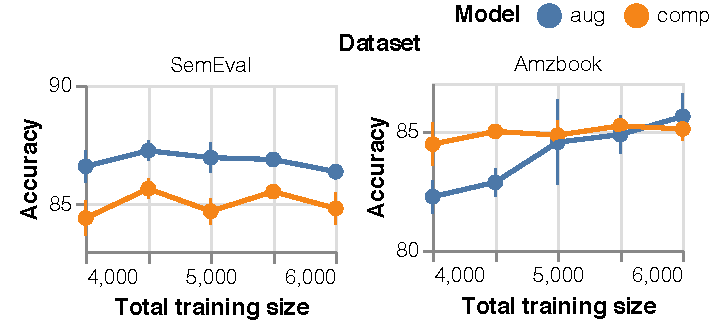
\includegraphics[width=1\columnwidth]{figures/sst_trend_2}
\vspace{-15pt}
\caption{The accuracy trend on \sst datasets, as the total training datasize $m+n$ varies. The blue line shows $m=2k$ \maug, and the orange one represents the corresponding \mcomp.
Though the counterfactuals remain useful on most datasets, too many counterfactuals may be harmful (\eg Amzbook when $m=n=2k$).
%\wts{Maybe cut/appendix?}
% (when $m+n=4k$, we have $m=n=2k$ on the orange line)
}
\vspace{-10pt}
\label{fig:sst_trend}
\end{figure}
\end{comment}


\definecolor{cfwone}{HTML}{eef5fa}
\definecolor{cfwtwo}{HTML}{daeaf5}
\definecolor{cfwthree}{HTML}{b2d2e9}
\definecolor{cfwfour}{HTML}{8abbde}

\newcommand{\fwone}[1]{\colbox{cfwone}{#1}\xspace}
\newcommand{\fwtwo}[1]{\colbox{cfwtwo}{#1}\xspace}
\newcommand{\fwthree}[1]{\colbox{cfwthree}{#1}\xspace}
\newcommand{\fwfour}[1]{\colbox{cfwfour}{#1}\xspace}

\newcommand{\fexp}[2]{\texttt{[{\color{darkgray}{#1:#2}}]}\xspace}
\newcommand{\fexptag}[1]{\fexp{TAG}{#1}}
\newcommand{\fexpfrom}[1]{\fexp{FROM}{#1}}
\newcommand{\fexpto}[1]{\fexp{TO}{#1}}
\newcommand{\fexptemp}[1]{\fexp{TEMP}{#1}}


\section{Counterfactual Explanations}

%Both counterfactual explanations and semi-counterfactual explanations.
%As defined in \cite{}

\subsection{Local explanations: Abnormality}





\begin{figure}[t]
\centering
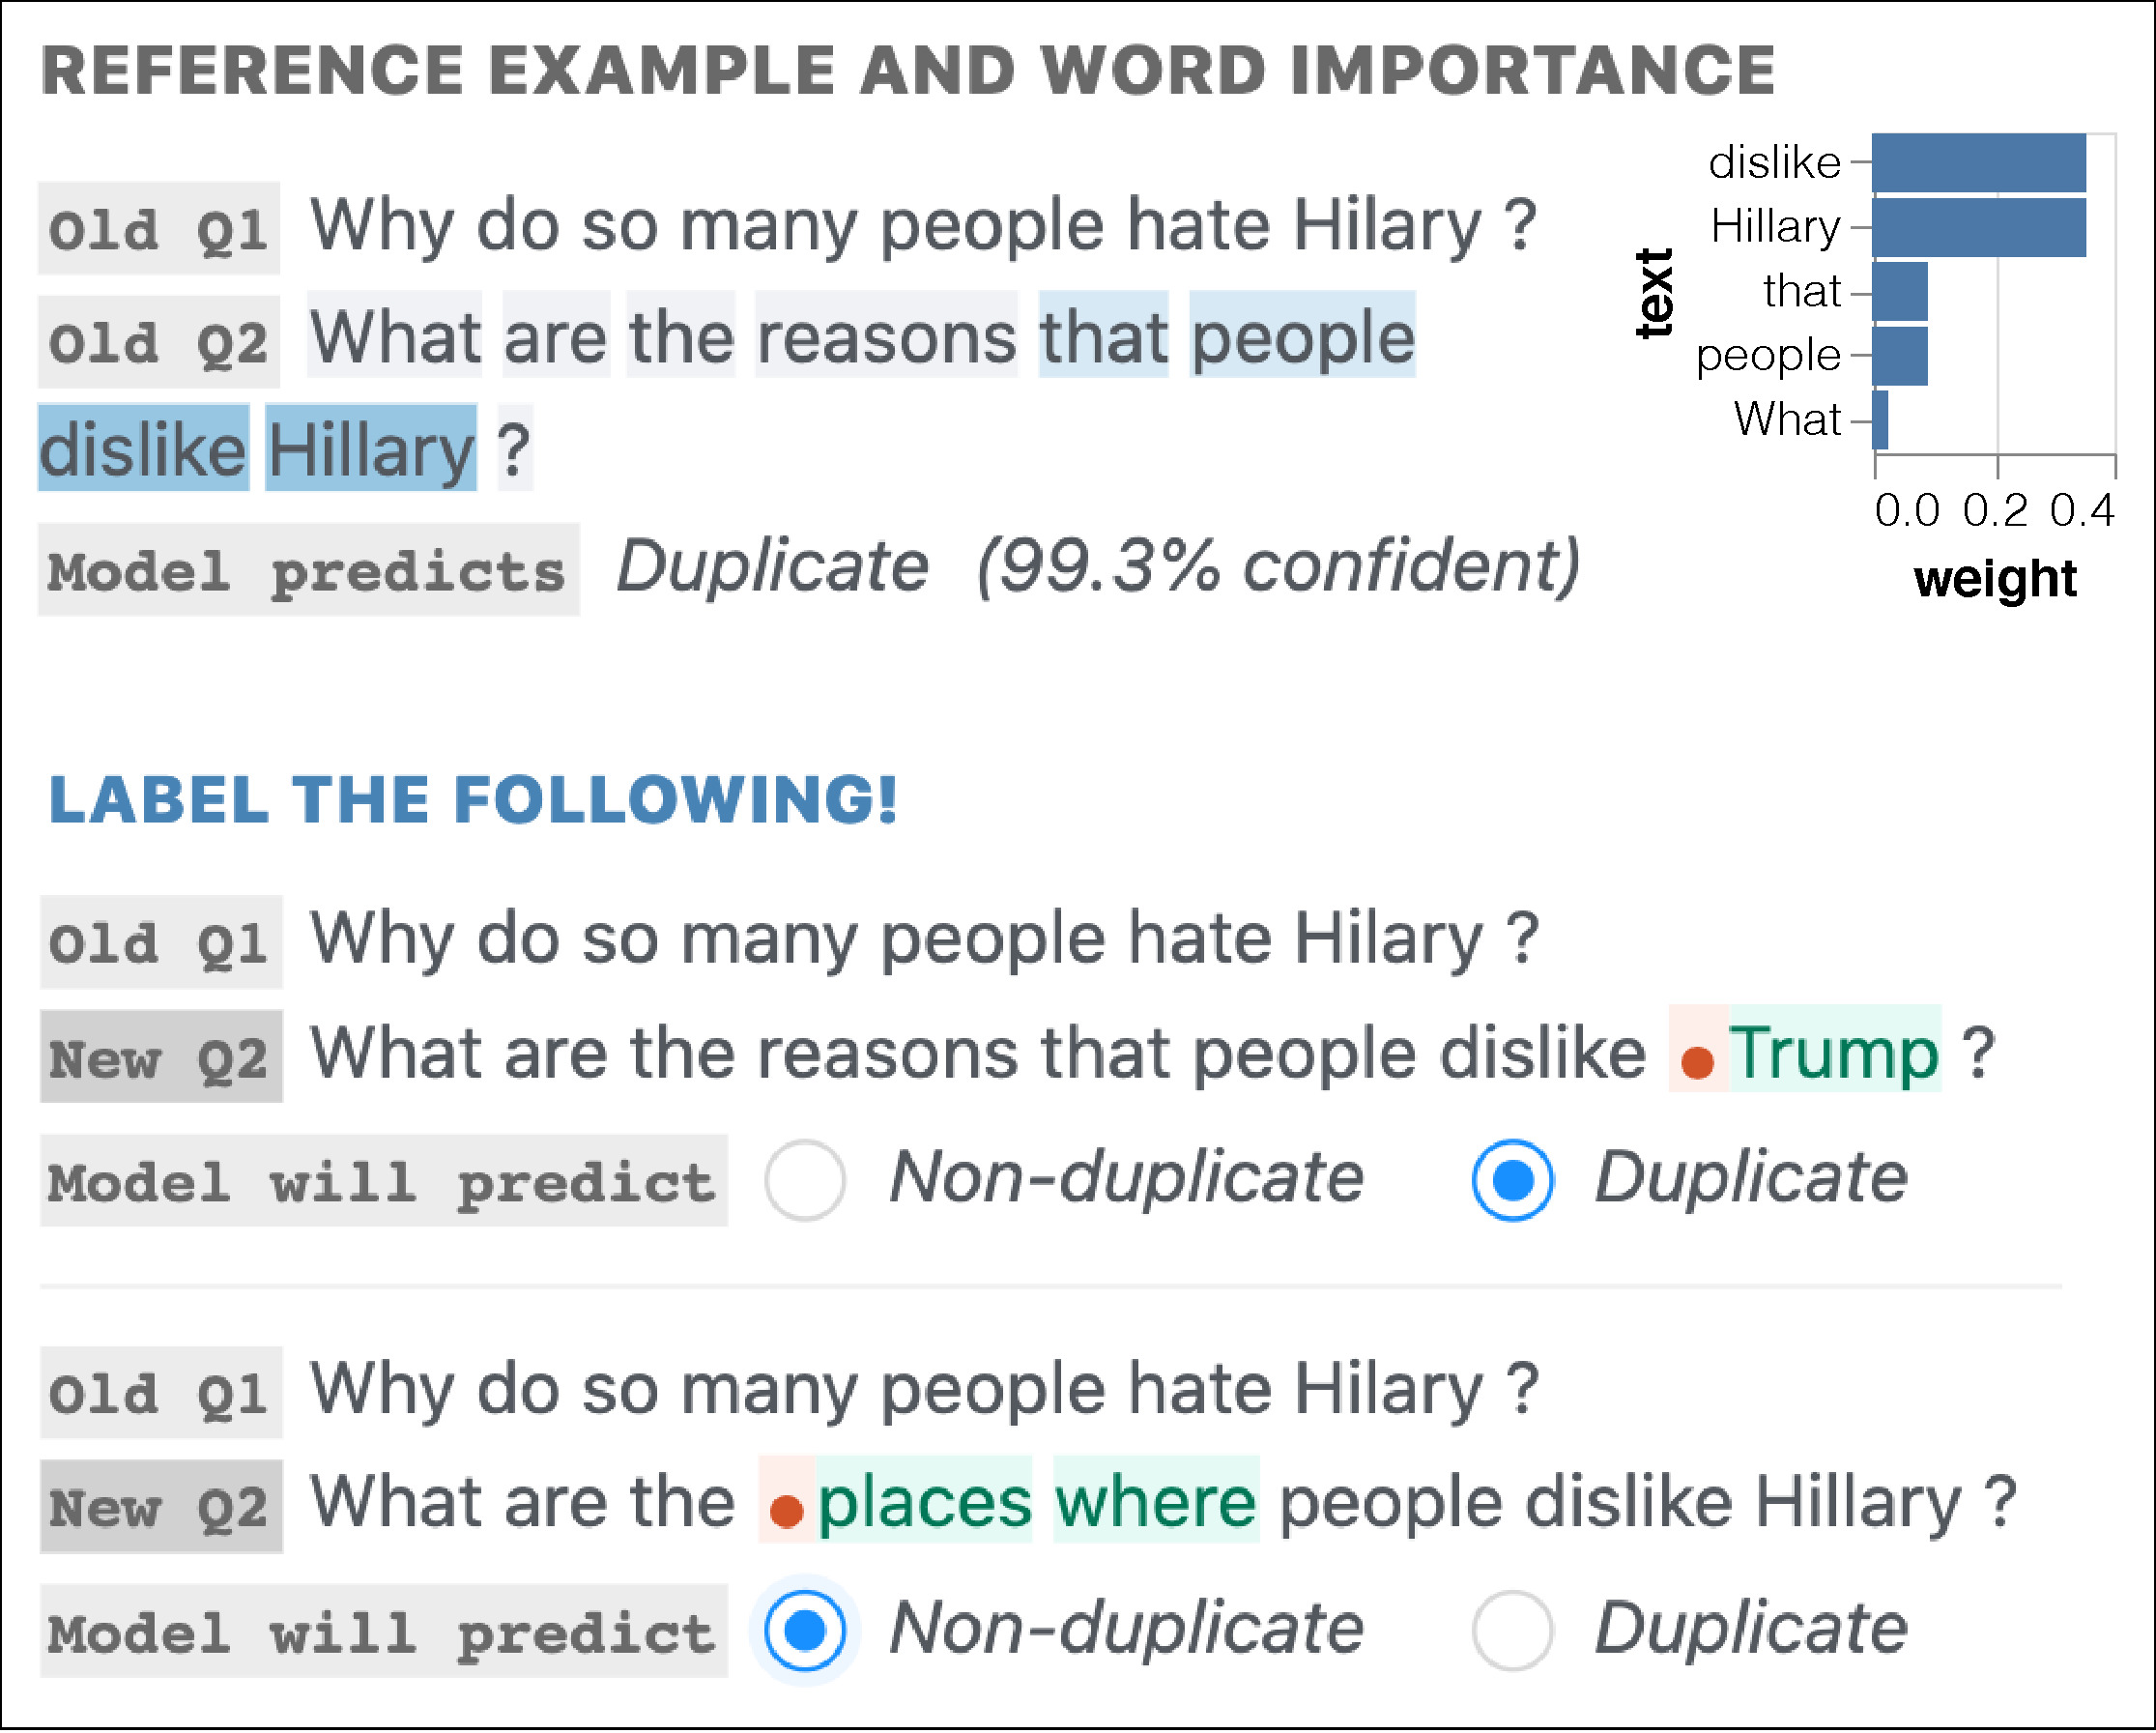
\includegraphics[width=1\columnwidth]{figures/explanation}
\vspace{-15pt}
\caption{}
\vspace{-10pt}
\label{fig:sst_trend}
\end{figure}



\wts{Finding bugs missed by the feature attribution, and concretizing the opaque weights using readable examples.}

\paragraph{Selection by abnormality.}
The cognitive burden of complete explanations is too great.
As a result, \citet{miller} concluded that people usually \emph{select} a small subset of (counterfactual) explanations on contrastive cases (``foils'') that they find unexpected. 
As such, he further proposed that ``abnormality could be used to infer likely foils.''
Here, we operationalize the concept of abnormality based on \emph{the discrepancy between the expected and the actual changes in the prediction}, and use it as our selection method.

Given a prediction model $f$, we define the actual change in prediction as $d_f(\xp, x)$, and the expected prediction change as $\hat{d}_f(\xp, x)$.
The distance between the expectation and reality then becomes:
$$\Delta d_f(\xp, x) = |\hat{d}_f(\xp, x)-d_f(\xp, x)|$$
We select two abnormal, ``turning point'' counterfactuals, \ie unexpected large changes in prediction when small (large) change is expected:
$$ \xp_l = \argmax_{\xp} \Delta d_f(\xp, x), \xp_s = \argmin_{\xp} \Delta d_f(\xp, x)$$
Whereas actual prediction change is always $d_f(\xp, x)=|f(\xp)-f(x)|$ where $f(x)$ denotes the prediction probability of $f$ on $x$, $d_f(\xp, x)$ can take various forms. 
For example, as a standalone explanation method, $\hat{d}_f$ can be the cosine distance in the \emph{Embedding space}.
The embedding can be either model-agnostic (\eg with~sentence transformers~\cite{reimers-2019-sentence-bert}), or the last layer of the hidden state of the finetuned predictor.

On the other hand, as a \emph{compensation} to existing feature attribution methods, $\hat{d}_f$ can be the importance (weights) of the perturbed tokens in $x$, estimated by feature attribution methods.
As mentioned in \wts{\S\ref{}}, methods like SHAP~\cite{} or LIME~\cite{} only estimate feature weights by \emph{masking} the words, which do not represent how model would react in non-deletion counterfactuals (replacing words or inserting negations).
Therefore, abnormalities selected in this way can  compensate or criticize the missed information, and therefore better calibrate users' trust on the predictor.
We primarily test the compensation selection below, as it nicely combines the overview provided by SHAP/LIME, and the decision boundaries omitted by the feature attribution. 
\wts{Add the detail to appendix?}



%%%%%%%
\subsection{Evaluate local explanations?}
We conduct a user study to verify whether our selected counterfactual explanations can compensate SHAP in helping people interpret the model, \ie if the selected counterfactual spot points that people would mis-interpret after viewing SHAP.
We form it as a model behavior simulation study, where participants are asked to predict model's behavior on the given counterfactuals.
Intuitively, the more counterfactuals they simulate incorrectly, the more information they grasp if we show the counterfactuals to them.

\paragraph{Procedure.}
We recruited \wts{N} graduate students who have experience using model explanations before, and asked them to simulate the behavior of a \qqp model for 20 rounds (the same as in \S\ref{subsec:contrast_set}).
In each round, the participants were given a reference example, with the model's prediction on it, its confidence score, as well as the feature attributions estimated by SHAP (\wts{Figure~\ref{}}).
To help them better understand the model around the reference example, the participants were allowed to ``query the model'' for up to 10 times, by making small changes to one question, and see the resulting model predictions.
It was equivalent to unlimited model access --- In the result, most participants submitted \wts{M} queries.
They were then asked to simulate the model's prediction on six counterfactuals, two from each condition.
After the 20 rounds, we concluded the study with open-ended questions on their model query and simulation strategies.

\paragraph{Conditions.} 
We compare three types of selected counterfactuals:
(1) \emph{SHAP-c}, the machine-generated counterfactuals selected to compensate SHAP; 
(2) \emph{random}, the randomly selected machine-generated counterfactuals; 
(3) \emph{human}, 
the human generated counterfactuals that they deemed abnormal.
We allowed three graduate students to play with the model for up to 10 times, and asked them to submit one final counterfactual with a surprising model prediction.
We then randomly selected two of their submissions per reference example.
As a within-subject study, we compared the error rate of human simulations across the three conditions.


\paragraph{Results.}
More interactions with the model usually results in better mental models about the predictor, and users wold become less surprised by most counterfactuals~\cite{miller}.
We are interested in learning whether our selected ones \emph{still add information}
Less surprised by abnormal phenomena, so an explanation alongside every decision runs the risk of providing explanations that become less needed and more distracting over time.

\begin{comment}
****
The examples generated by BERT.
****

  P: The quarterback of the UTEP football team is about to be tackled by a member of the Wisconsin defensive team.
  H: The quarterback is about to be tackled by the opposing team.
 Pr: entailment
 NP: Another quarterback is about to be tackled by the opposing team.
NPr: neutral
weight:  0.122
flip_unimportant_feature 0.013 {The}

  P: The quarterback of the UTEP football team is about to be tackled by a member of the Wisconsin defensive team.
  H: The quarterback is about to be tackled by the opposing team.
 Pr: entailment
 NP: Jack is about to be tackled by the opposing team.
NPr: neutral
weight:  0.461
flip_unimportant_feature 0.028 {The, quarterback}


  P: The quarterback of the UTEP football team is about to be tackled by a member of the Wisconsin defensive team.
  H: The quarterback is about to be tackled by the opposing team.
 Pr: entailment
 NP: The quarterback is about to be tackled by someone
NPr: entailment
weight:  0.218
unflip_important_feature 0.3 {team, the, ., opposing}

  P: The quarterback of the UTEP football team is about to be tackled by a member of the Wisconsin defensive team.
  H: The quarterback is about to be tackled by the opposing team.
 Pr: entailment
 NP: The quarterback is about to be tackled by the second team.
NPr: entailment
weight:  0.292
unflip_important_feature 0.149 {opposing}


\end{comment}


\subsection{Global / Interactive Explanations}
\label{subsec:global_exp}
Here, we explore more extensive use of perturbation explanations via examples, but defer more sophisticated designs and evalautions to future work.

\paragraph{Global explanations: impacts of same changes.}
Going beyond turning points for each individual data points, we can find perturbation patterns that systematically affect (preserve) model predictions.
Similar to challenge sets, the grouped perturbations then become useful for revealing model's capabilities on specific linguistic patterns.

To enable the grouping, we first featurize each perturbation $\xp$ with respect to its original instance $x$, using 
(1) its \tagstr (\fexptag{negation} for the example in Figure~\ref{fig:blank}), 
(2) its remove phrases \fexpfrom{kids}, 
(3) its added phrases \fexpto{not}, \fexpto{children}, and 
(4) the combined template \fexptemp{\swap{kids}{children}}.
For tokens involving multiple changes, we featurize both the primary and the combined changes, and so the example in Figure~\ref{fig:blank} also have additional features like \texttt{\fexptag{negation} \& \fexptag{lexical}}.

For each feature $h$ we compute the its prediction change rate over all the perturbations $\xp \in \xset_{h}$ that have the said feature: 
$R_h = \sum {\mathbb{1}[f(x) \not\eq f(\xp)]} / |\xset_h|$.

Filters on the change rate then reveal different model prediction patterns.\footnote{Because different \nli labels follow very flip patterns, we only include $f(x)=entailment$ examples here}

\noindent\textbf{Mastered patterns.}
Patterns with very high or low change rates (\eg $|R_h-0.5| > \gamma=0.3$) reveal patterns that the model has firmly learned.
In \nli, it includes \fexptemp{\swap{men}{women}} ($R_h=97\%$), \fexptemp{\swap{outdoor}{outside}} ($R_h=0\%$).

\noindent\textbf{Outliers.}
Inspecting the abnormal cases in \emph{mastered patterns}, we find harder to notice examples.
\fexptemp{\swap{three}{four}} changes the 80\% prediction(on 56 changed examples), but all the cases with affected predictions have the explicit pattern ``three'' in the premise, whereas the prediction intact ones show that the model has a hard time processing the actual counting.

\ebox{
\textbf{P}: Three girls fell on top of one another and are laughing.\\
\textbf{H}: \swap{Three}{Four} girls falling and laughing.\\
\textbf{Pr}: \swap{entailment}{contradiction}\\

\textbf{P}: Two little girls and one little boy are running.\\
\textbf{H}: \swap{Three}{Four} kids are running. \\
\textbf{Pr}: \swap{entailment}{entailment}
}

\noindent\textbf{Missed patterns.}
In contrast of the mastered cases, patterns with mild change rates (\eg $|R_h-0.5| < \gamma=0.2$) reveal patterns that the model handles unstably.
For example, the model does not handle the shuffled phrases, echoing the results from \citet{mccoy2019right}.

\ebox{
\fexptag{shuffle}, $R=0.63$ (164 cases)\\
\textbf{P}: The bride in the white dress is surrounded by the groomsmen and bridesmaids, all in black.\\
\textbf{H}: \add{white} woman \remove{in white} is surrounded by others.\\
\textbf{Pr}: \swap{entailment}{entailment}\\

%\textbf{Premise}: Man juggling apples while sitting on a couch with another man on one side and a woman on the other.\\
%\textbf{Hypothesis}: Two \swap{men}{women} sitting near a \swap{woman}{man}.
%\textbf{Prediction}: \swap{entailment}{entailment}\\

\textbf{P}: A man in a wheelchair is being pushed towards a monk.\\
\textbf{H}: The \swap{person is disabled and}{holy person} is being moved towards a \swap{holy}{disabled} person. \\
\textbf{Pr}: \swap{entailment}{entailment}
}


\paragraph{Interactive explanation.}
Besides pre-selected \emph{surprise} cases, perturbations can also support interactive explanation (ideally in a visual interface), and multi-step drill downs.
In the example: 

\ebox{
\textbf{P}: Some dogs are running on a deserted beach.\\
\textbf{H}: There is only one dog at the beach.\\
\textbf{Pr}: contradiction
}

To understand whether the model responses to quantifiers, an analyst can \BLANK ``only one'', which would reveal that the model predicts entailment correct for both perturbed hypotheses:

\ebox{
\textbf{H}: There \swap{is only one dog}{are multiple dogs} at the beach.\\
\textbf{H}: There is \swap{only}{more than} one dog at the beach.
}

Then, the analyst can keep ``more than one dog'' to inspect how the model react to other changes. 
With the model maintaining entailment on the following examples, the analyst would conclude that there may be a strong correlation between NNS and ``more than one,'' that it overwrites many of the prep constraints.

\ebox{
\textbf{H}: There is \emph{more than} one dog at the beach \add{lying down}.\\
\textbf{H}: There is \emph{more than} one dog at the beach \add{inside a cup}.\\
\textbf{H}: There is \emph{more than} one dog at the beach \add{standing}.
}


\section{Related Work}
\label{sec:relate}

Some prior work in counterfactual training and evaluation relies on humans to generate counterfactuals from scratch~\cite{gardner2020contrast, teney2020learning, kaushik2019learning}. 
Our experiments in \S\ref{sec:app_label} indicate that a hybrid approach where humans \emph{label} \sysname{} counterfactuals displays similar or better results at a much lower cost, and that it may be worth exploring a mixture of manual and automated generation. 
Similarly, prior work on analysis relies on experts to create individual counterfactuals or perturbation functions~\cite{wu2019errudite, checklist:acl20}. 
In \S\ref{sec:app_err_analysis}, we show how \sysname{} can enhance current practice by generating multiple counterfactuals that might have been overlooked, and by providing abstractions that allow for new kinds of analyses.

At the other end of the spectrum, prior work on automatically generating counterfactuals typically narrows its scope in terms of the relationships $x \veryshortarrow \xp$.
For example, adversarial generators aim to maintain semantics while changing model predictions~\cite{ribeiro2018semantically, iyyer2018adversarial, alzantot-etal-2018-generating}.
Meanwhile, concurrent work to our own~\cite{madaan2020generate, ross2020explaining} automatically generate $\xp$ that change predictions for the purpose of explanation or training, with no constraints on semantics.
However, as many of our examples in \S\ref{sec:app_label}--\S\ref{sec:app_err_analysis} show, a mix of label-preserving and label-flipping counterfactuals generated by \sysname is quite useful for training, evaluation, explanation, and analysis. 
Further, general-purpose counterfactuals may lead to serendipitous discoveries (\S\ref{sec:app_err_analysis}), especially as \sysname is not fine-tuned to the target domain (and thus less liable to merely replicate what is already there).
Finally, by allowing control through \tagstrs and \texttt{[BLANK]}s, \sysname{} supports human-generator collaborations, where the human specifies the desired changes (\eg change predictions \emph{through negation}).
Such collaboration is difficult to imagine with automatic generators.
Similarly, editing-based text style transfer only perturbations based on predefined style attributes~\cite{madaan-etal-2020-politeness, malmi-etal-2020-unsupervised}, with no finer-grained controls.


% Counterfactuals in various applications differ by their impact on the groundtruth and model prediction labels.
% Those changing the groundtruth are mostly used for counterfactual training~\cite{kaushik2019learning, teney2020learning} and evaluation~\cite{gardner2020contrast, checklist:acl20}.
% As mentioned in \S\ref{sec:intro}, these counterfactuals rely heavily on human creativity and are expensive to collect.
% Though it is cheaper to automate the process with parsing templates~\cite{li2020linguistically}, usually the templates are only applicable to a small subset of data.
% \citet{wang2020robustness} also proposed to automatically flip the groundtruth by replacing causal word features with their antonyms.
% However, they acknowledged that the method supplies limited tasks, as ``antonym'' is only well-defined in sentiment analysis.
% We achieve a middle ground, showing that the team of \sysname and a human moderator collect data more effectively.

% On the other hand, multiple prior works automatically generate counterfactuals that flip model predictions.
% These methods are used for counterfactual explanations.
% For example, \citet{kang2020counterfactual} guided word replacement with model prediction probabilities.
% Our concurrent work, GYC~\cite{madaan2020generate} and MiCE~\cite{ross2020explaining} further enable phrase replacement through language models (GPT-2 or t5).
% However, these methods leave out prediction-persistent explanations, which are also important as shown in \S\ref{sec:app_explain}.
% If collected with additional constraints on semantic persistence~\cite{morris2020textattack, alzantot-etal-2018-generating}, the prediction-flipping counterfactuals become adversarial examples.
% Despite the apparent similarities between explanations and adversarials, to the best of our knowledge, adversarial generation is still mostly through word replacement~\cite{alzantot2018generating, garg2020bae, li2020contextualized} or paraphrasing~\cite{iyyer2018adversarial, malandrakis-etal-2019-controlled}, and has yet to take advantage of language models.
% Given the shared properties, a general-purpose model like \sysname may be more reasonable than methods tailored to specific applications.

% Moreover, the emphasis on \emph{labels} compresses a large set of diverse changes (\eg negations and antonym replacements both flip labels in sentiment analysis), and therefore hinders the definition and queryiig of desired counterfactuals.
% We instead design \sysname's controls to be task (label)-agnostic and finer-grained.
% Such controls additionally support applications that require specifications on where and how to perturb, \eg open-ended error analysis~\cite{wu2019errudite} where contrasting similar counterfactuals is essential (\S\ref{sec:app_err_analysis}).



\section{Discussion and Conclusion}
\label{sec:discuss}

We propose \sysname, an automated method for general-purpose counterfactual generation. 
As a text generation task, \sysname takes in a sentence, as well as (optionally) \tagstrs and blanks as the prompt.
It outputs corresponding counterfactuals, which can be further filtered for different downstream use cases. 
We show that the \sysname can support counterfactual data augmentation, contrast set generation, as well as counterfactual explanation.
Below, we discuss promising future work:

\textbf{Supporting existing counterfactual reasoning tools.}
Besides independent use cases, \sysname can also support existing tools for data programming, model testing and error analysis.
For example, featurizing counterfactuals into Snorkel labeling functions~\cite{ratner2017snorkel} helps collect the training and evaluation data more efficiently (similar to \S\ref{subsec:global_exp}).
Or, domain experts can create perturbation tests more easily if \sysname serves as an additional building block for Errudite~\cite{wu2019errudite} or CheckList~\cite{checklist:acl20}.


\textbf{Human-in-the-loop Counterfactual Generation.}
Besides placing blanks and labeling counterfactuals, humans can add more values when they actively collaborate with \sysname.
For example, human creators can increase the diversity of the covered patterns, if they are asked to come up with more counterfactuals that are different from those covered automatically.
In tasks that require context-dependent counterfactual generations, human annotators can also initiate seed counterfactuals for \sysname to extend.
For example, \citet{gardner2020contrast} perturbed multi-hop question answering by adding compositional reasoning steps \emph{related to} the corresponding paragraph.
Such context- and logic- aware perturbations are hard for the model alone; however, it can further perturb the reasoning step \emph{once} the human adds it into the sentence.



\bibliography{ref}
\bibliographystyle{acl_natbib}

\clearpage
\newpage

\appendix
\section{Datasets for GPT-2 Finetuning}
\label{appendix:train_data}

%\begin{comment}
\begin{table*}
\small
\centering
\setlength{\tabcolsep}{3.5pt}
\begin{tabular}{lrrrrrrrrr}
\toprule
\textbf{Dataset} & \textbf{\ctrltag{negation}} & \textbf{\ctrltag{quantifier}} & \textbf{\ctrltag{leixcal}} & \textbf{\ctrltag{resemantic}} & \textbf{\ctrltag{insert}} & \textbf{\ctrltag{delete}} & \textbf{\ctrltag{restructure}} & \textbf{\ctrltag{shuffle}} & \emph{\ctrltag{global}} \\ 
\midrule
        CAD &      3418 &         435 &     7335 &        3896 &    2430 &    2432 &         3872 &       82 &    3702 \\
    Crawled &         0 &           0 &     5000 &           0 &    5000 &    5000 &            0 &       91 &    5000 \\
   contrast &       314 &         294 &     1180 &        1167 &     575 &     575 &         1085 &      113 &     843 \\
       hans &        46 &           0 &        0 &           0 &    3893 &    3891 &          791 &     1180 &     199 \\
    paranmt &      2201 &         513 &     5262 &       10000 &    5446 &    5400 &        10000 &     1592 &   10000 \\
       paws &        61 &         284 &     5672 &        2732 &    4161 &    4155 &        10000 &    10000 &   10000 \\
 winogrande &      3134 &         116 &    10000 &        7612 &     169 &     170 &         4271 &      233 &    3395 \\
      total &      9174 &        1642 &    34449 &       25407 &   21674 &   21623 &        30019 &    13291 &   33139 \\
\bottomrule
\end{tabular}
\caption{The datasets used for finetuning the GPT-2 perturbation model, and the \tagstr distributions.}
\label{table:gpt_train_stats}
\end{table*}
%\end{comment}


We combined the following NLP datasets in finetuning our GPT-2 perturbation model.
To achieve a more balanced distribution, for each dataset, we extract \tagstrs from all the data pairs available, and randomly sample up to 10k instances per \tagstr.
The distribution is shown in Table~\ref{table:gpt_train_stats}.

\paragraph{Contrast set}
In \cite{gardner2020contrast}, authors of 10 existing NLP dataset each manually perturbed 100-1,000 test instances in small but meaningful ways that change the gold label, so to inspect a model's decision boundary around a local instance.
\wts{Make sure NLP is expanded somewhere in intro}
The perturbation pattern varies based on the tasks and the annotators, allowing us to learn diverse perturbation methods.
To make sure we can use the contrast set to evaluate the sentiment analysis model, we excluded the IMDB movie review from the training.
\footnote{Similarly, though QQP would be a potentially interesting dataset for training the perturbation model, we omitted it so QQP can be used in our evaluation.}
%\wts{Re-train the model with other contrast sets.}


\paragraph{Counterfactually-augmented data (CAD)}
To augment the training data, \citet{kaushik2019learning} crowdsourced counterfactual perturbations for IMDB movie review (1.7k perturbations on 1.7k original instances) and SNLI (6.6k perturbations on 1.67k original instances).
Similar to contrast set, the perturbation patterns vary based on the task, but can especially contribute to \ctrltag{negation}.
We split the movie review paragraphs into paired sentences, to match the sentence length of other datasets.


\paragraph{WINOGRANDE} is a large-scale dataset of 44k problems for testing common sense problems~\cite{sakaguchi2019winogrande}.
The dataset contains nearly identical sentences that differ only by one trigger word, which flips the correct answer choice for certain questions.
The dataset is most suitable for lexical tokens that are suitable for similar use cases.

\paragraph{ParaNMT-50M} contains 50 million English-English sentential paraphrase pairs, covering various domains and styles of text, as well as different sentence structures~\citet{wieting2017paranmt}. 

\paragraph{PAWS} contains paraphrase and non-paraphrase pairs with high lexical overlap. 
\citet{zhang2019paws} created 108k challenging pairs by controlled word swapping and back translation.
As a result, the dataset demonstrates the \ctrltag{shuffle} and \ctrltag{restructure} strategy.


\paragraph{HANS} is a controlled evaluation dataset designed for testing decision boundaries of NLI models~\cite{mccoy2019right}. 
The dataset contains 10k pairs of premises and hypotheses created based on 10 heavily on fallible syntactic heuristic rules, and therefore compensates rarer structural changes that may be missed by PAWS.


\paragraph{Crawled} 
\wts{Explain why we included the crawled and why only some columns.}



\section{Survey of Perturbation Applications}

A table summarizing the papers, the perturbation strategies.
Maybe need to separate the manual types.

\begin{comment}
	\begin{table}
\small
\centering
\setlength{\tabcolsep}{3.5pt}

\begin{tabular}{c c c c c}
\toprule
Application & \textbf{$y'\not\eq y$} & $f(x) \not\eq f(x')$? & Strategies & Properties \\ 
\midrule
Augmentation & \cmark & \qmark & Paraphrasing & Natural; Diverse \\
\bottomrule
\end{tabular}

\caption{The datasets used for finetuning the GPT-2 perturbation model, and the \tagstr distributions.}
\label{table:gpt_train_stats}
\end{table}
\end{comment}


\section{Labeling Instructions \& Quality}
\label{appendix:label_instruct}


\begin{figure*}[h]
\centering
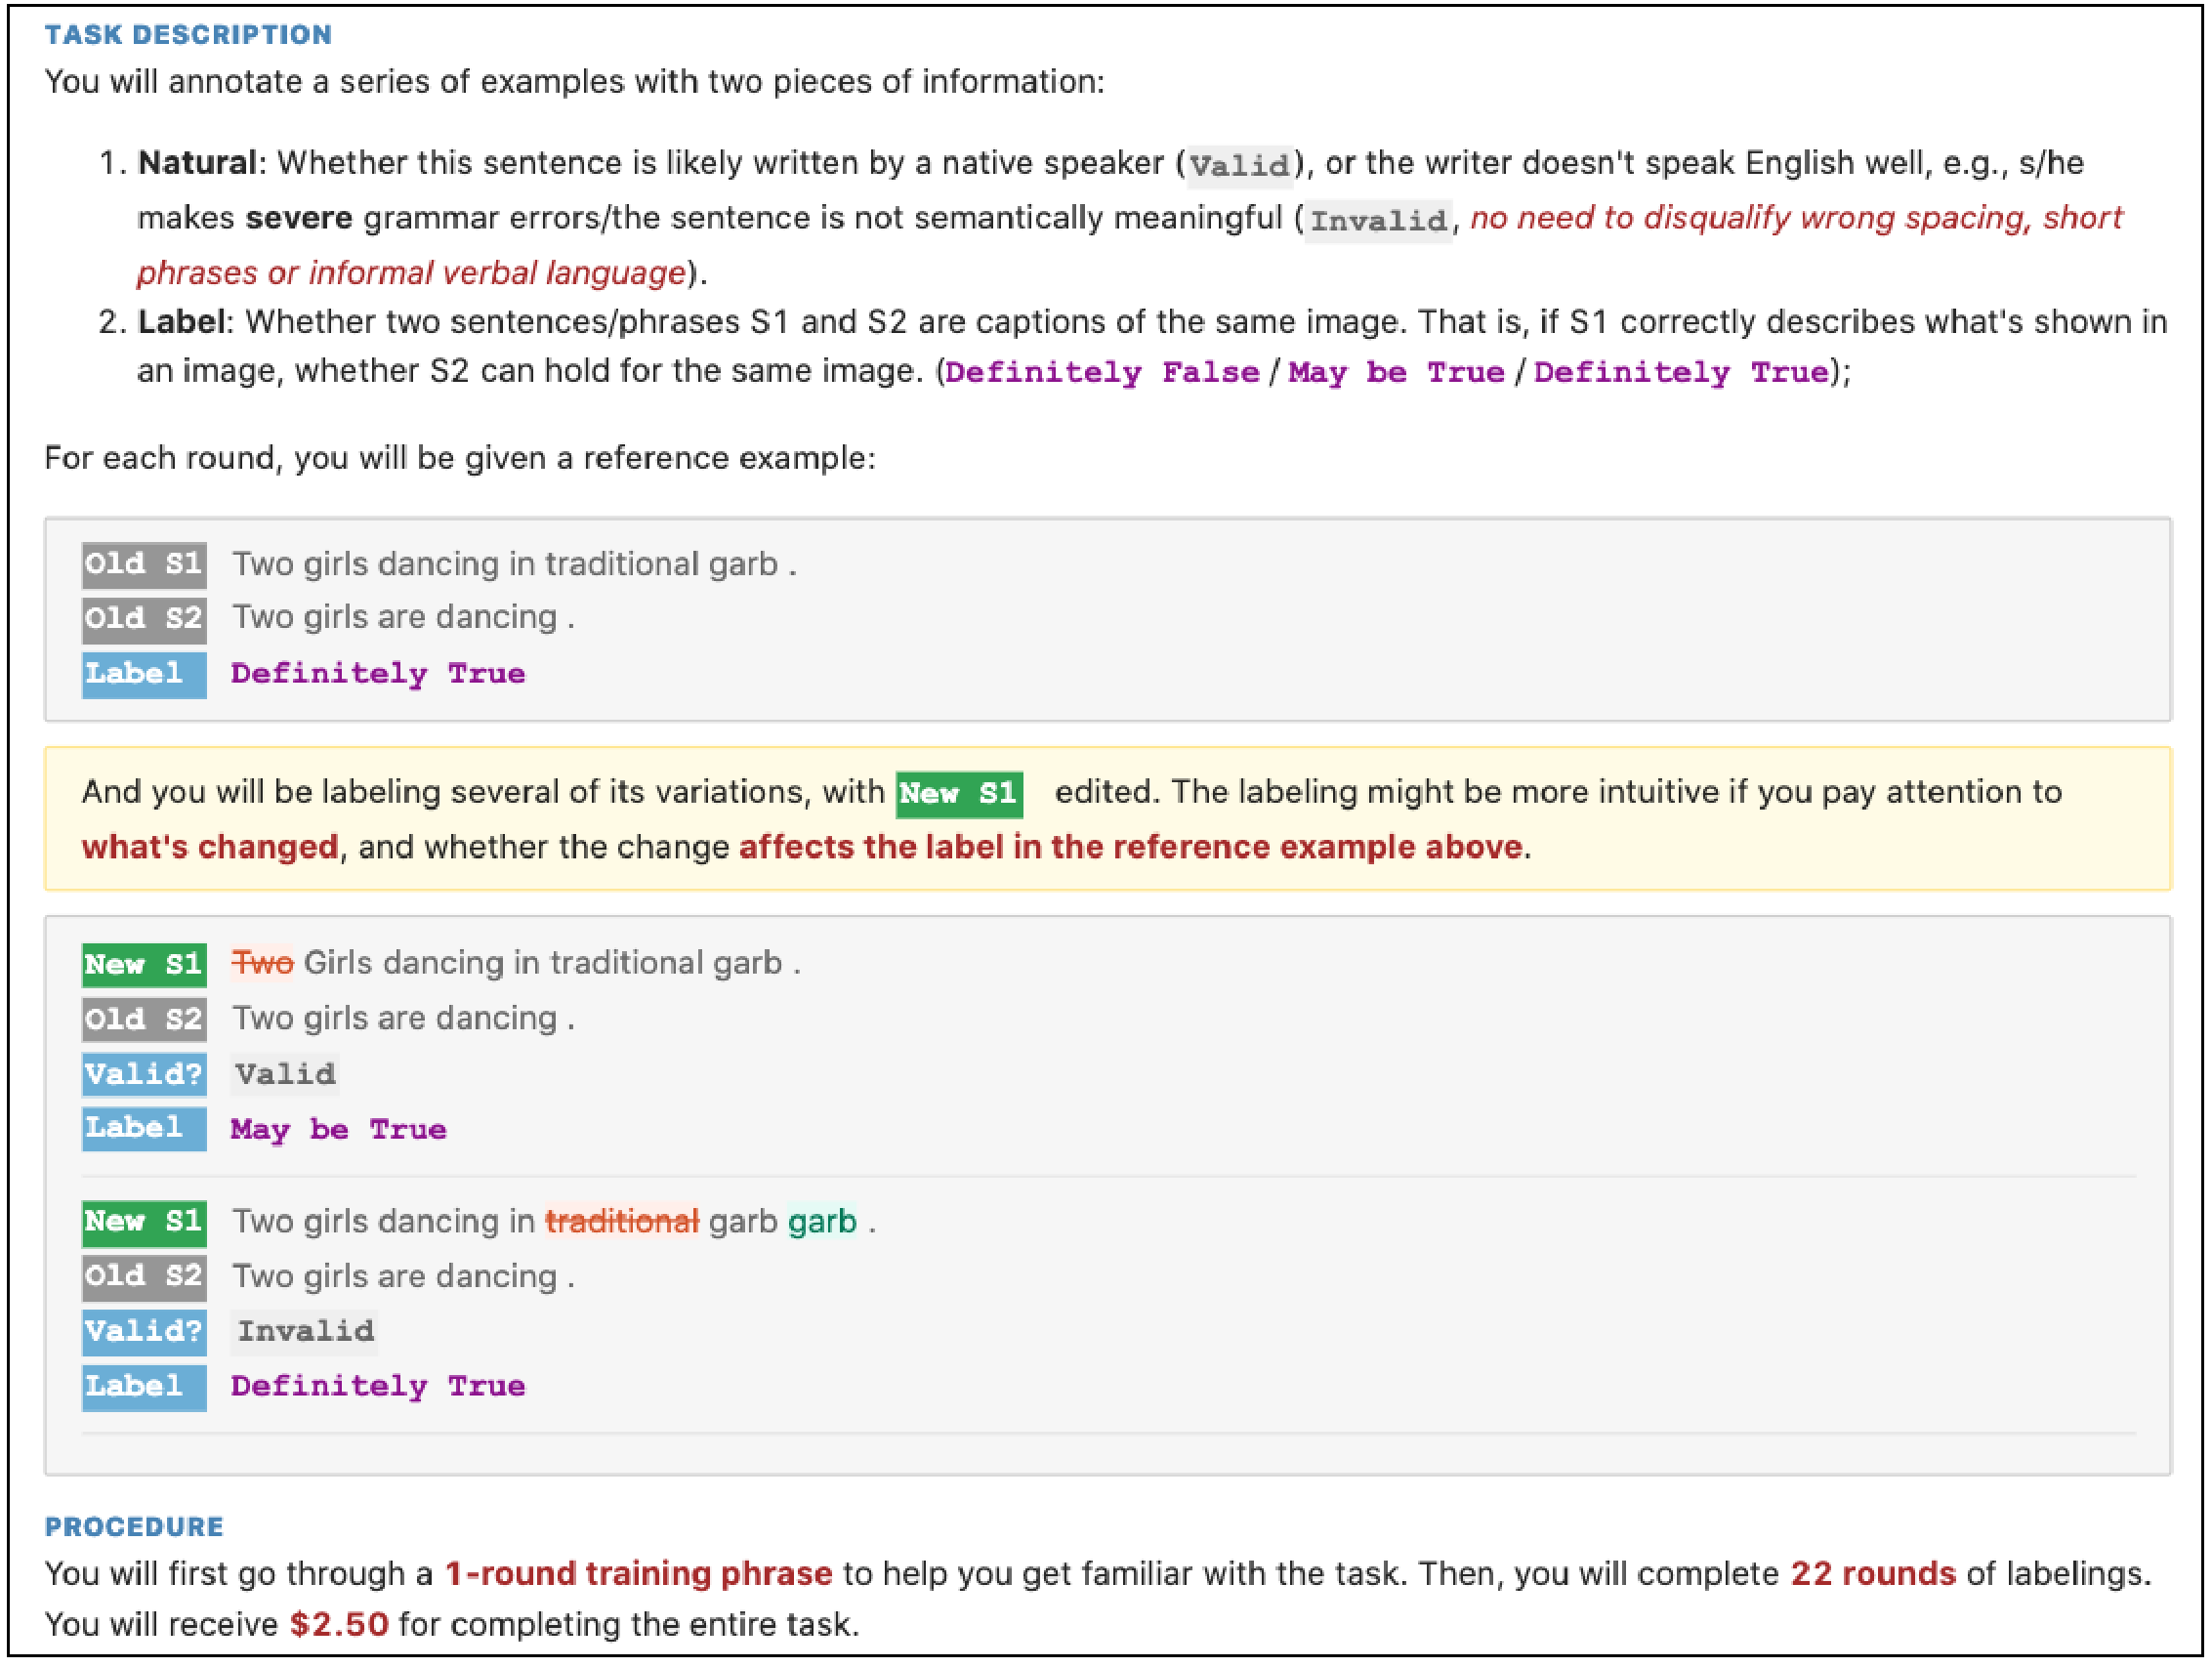
\includegraphics[width=1\textwidth]{figures/mturk_instruction.pdf}
\vspace{-15pt}
\caption{A sample instruction for the \nli task, with annotators providing labels based for the perturbed hypotheses (\emph{New S2}). Instructions are similar for \qqp and \sst, except for the label definitions and the examples. \wts{Change to hypothesis screenshot.}}
\vspace{-10pt}
\label{fig:mturk_instruction}
\end{figure*}

\paragraph{Procedure\footnote{A complete annotation demo is available at \mturkurl.}}
The study started with an introduction, in which we explained the context and tasks (Figure~\ref{fig:mturk_instruction}): 
``given a reference example, the crowdworker should annotate its perturbed variations, based on whether the perturbation is valid (\emph{sounds natural}), and the classification task label.''
To familiarize them with the task, we asked them to complete 1-2 training rounds, and explained the expected labels.
The annotator then completed 22 tasks, each labeling 3 variations of a single example.
The 22 rounds consisted of 20 actual labeling tasks and 2 extra ``gold rounds'' (6 labeled examples), with unambiguous examples and known groundtruth labels, which later served as filters for high quality crowdworkers.
As a result, each annotator contributed $20 \times 3=60$ labels.
The median task completion time was around 15-20 minutes (14.9 for \qqp, 16.7 for \sst, and 19.8 for \nli), and participants received an average payment of \$2.5 (equivalent to an hourly wage of \$7.5).

\paragraph{Participants}
We recruited participants from Amazon's Mechanical Turk (MTurk), limiting the pool to subjects from within the United States with a prior task approval rating of at least 97\% and a minimum of 1,000 approved tasks.

\paragraph{Data quality}
We applied two filtering strategies: 
(1) \emph{High quality worker.} 
We only kept data from participants whose median labeling time was more than 18 seconds and correctly labeled at least 4 gold examples (out of 6), or who correctly labeled all gold ones.
(2) \emph{Majority vote labeling.}
We collected two annotations per perturbation, and only kept data points that at least one annotator deems \emph{valid}, and both annotators agree on a particular \emph{class label.}

As such, when set out to collect augmentations on 1,000 original examples (thus 3,000 perturbations), we typically collect perturbations for 1,000 perturbations on 600 original examples.
One of the authors labeled a subset of 100 perturbations on 100 original examples in \sst, and reached high agreement with the majority-voted results ($\kappa=0.77$, the raw labeling agreement $88\%$).




\begin{table*}[bp]
\small
\centering
\begin{tabular}{p{0.95\linewidth}}
\toprule
\textbf{Additional examples} \\ 
\midrule
It sucked \add{me in}. \\
\midrule

For those who are intrigued by politics of the '70s , the film is every bit as \swap{fascinating}{flawed} as it is \swap{flawed}{intriguing}. \\
\midrule

So exaggerated and broad that it comes off as \swap{annoying}{engaging} rather than \swap{charming}{annoying}. \\
\midrule

The film \swap{delivers}{doesn't deliver} what it promises: A look at the ``wild ride'' that ensues when brash young men set out to conquer the online world with laptops, cell phones and sketchy business plans. \\
\midrule

It's a crime movie made by someone who obviously knows \swap{nothing}{much} about crime. \\
\midrule

\swap{Even with}{Despite} all its botches, Enigma offers \swap{all}{none of} the pleasure of a handsome and well-made entertainment .\\
\midrule

``Catch Me'' feels \add{almost} capable of charming the masses with star power, a pop-induced score and sentimental moments that have become a Spielberg trademark.\\
\midrule

A sentimental but entirely \swap{irresistible}{unentertaining} portrait of three aging sisters.\\
\midrule

This is a movie full of \swap{grace}{mistakes} and, ultimately, \add{no} hope.\\
\midrule

Its simplicity puts an exclamation point on the fact that this isn't something to be taken seriously, but it also \swap{wrecks any chance}{poses an opportunity} of the movie rising above similar fare.\\
\midrule


\swap{If}{Even if} the film \swap{fails to fulfill}{succeeds in fulfilling} its own ambitious goals , it \swap{nonetheless sustains}{fails to sustain} interest during the long build-up of expository material .\\

\bottomrule
\end{tabular}
\vspace{-5pt}
\caption{Additional examples for Sentiment Analysis.}
%\wts{Change all the examples to be on an identical sentence, not all different cases. And consider further annotate the tags based on whether they just do semantic change or also syntactic change.}}
\label{table:sst_example}
\vspace{-10pt}
\end{table*}


\begin{table*}[bp]
\small
\centering
\begin{tabular}{p{0.95\linewidth}}
\toprule
\textbf{Additional examples} \\ 
\midrule


\textbf{Q1}: Poor people are more generous than rich people. Why? \newline
\textbf{Q2}: Is it true \swap{poor}{rich} people are more generous than \swap{rich}{poor} people? \\
\textbf{Q2}: Is it true poor people \swap{are more generous}{give more to charities} than rich people? \\
\midrule

\textbf{Q1}: Are TripAdvisor reviews more reliable than Yelp reviews because of their review process \newline
\textbf{Q2}: Are TripAdvisor reviews \swap{more}{less} reliable than Yelp reviews? \newline
\textbf{Q2}: Are TripAdvisor reviews more \swap{reliable}{unreliable} than Yelp reviews? \newline
\textbf{Q2}: Are \swap{TripAdvisor}{Yelp} reviews more reliable than \swap{Yelp}{TripAdvisor} reviews? \\
\midrule

\textbf{Q1}: How do you describe a smell? \newline
\textbf{Q2}: How will you describe a smell \swap{to}{from} a person? \newline
\textbf{Q2}: How will you describe a \swap{sound}{smell} to a person? \\
\midrule

\textbf{Q1}: Why are most psychopaths males and not females?and are female psychopaths different from male psychopaths? \newline
\textbf{Q2}: Is there a difference between male \remove{and female} psychopaths? \newline
\textbf{Q2}: Is there a difference between male and female \remove{psychopaths}? \newline
\textbf{Q2}: \add{Why} is there a difference between male and female psychopaths? \\
\midrule

\textbf{Q1}: How can I loose 5kgs weight in a week without exercise? \newline
\textbf{Q2}: How can I lose weight \swap{without}{by} doing exercise? \newline
\textbf{Q2}: How can I lose weight \remove{without doing exercise}? \newline
\textbf{Q2}: \swap{How can I}{Why can't you} lose weight without doing exercise? \\

\bottomrule
\end{tabular}
\vspace{-5pt}
\caption{Additional examples for Duplicate Question Detection, with the Q1 intact and Q2 changed.}
%\wts{Change all the examples to be on an identical sentence, not all different cases. And consider further annotate the tags based on whether they just do semantic change or also syntactic change.}}
\label{table:qqp_example}
\vspace{-10pt}
\end{table*}


\begin{table*}[bp]
\small
\centering
\begin{tabular}{p{0.95\linewidth}}
\toprule
\textbf{Additional examples} \\ 
\midrule

\textbf{P: }A small child stands in front of short white table.\newline
\textbf{H: }A child \swap{near}{sitting on} a table.\\
\midrule


\textbf{P: }A child sticks his head through a hole to create a picture of his head being a flower blossom\newline
\textbf{H: }The child is poking his head \swap{through}{to see} something.\\
\midrule

\textbf{P: }A young woman is playing fool.\newline
\textbf{H: }The woman is \swap{old}{very young} and not playing any games.\\
\midrule

\textbf{P: }Metal supports make a repeating X shape along the wall of the station.\newline
\textbf{H: }The walls are stronger with \swap{metal}{wood} supports rather than \swap{wood}{metal fences}.\newline
\textbf{H: }The walls are \swap{stronger}{less sturdy} with metal supports rather than wood.\\
\midrule

\textbf{P: }Several gentlemen are speaking into a microphone and the man in the glasses appears to be saying something funny\newline
\textbf{H: }Somebody \swap{that is shown wears}{shows} glasses.\\

\bottomrule
\end{tabular}
\vspace{-5pt}
\caption{Additional examples for Natural Language Inference, with the \textbf{P}remise intact and \textbf{H}ypothesis changed.}
%\wts{Change all the examples to be on an identical sentence, not all different cases. And consider further annotate the tags based on whether they just do semantic change or also syntactic change.}}
\label{table:nli_example}
\vspace{-10pt}
\end{table*}


\section{Additional counterfactuals}
\label{appendix:example}
Here, we include some additional counterfactual for each classification task.

%\section{Computing the Pturbation Similarity}
%\label{appendix:perturb_similarity}

\end{document}
